%\documentclass[overheadsbeamer.tex]{subfiles}
\documentclass[handoutsbeamer.tex]{subfiles}

\begin{document}

\thispagestyle{empty}

\ona{ \setcounter{chapter}{7} } % ONE LESS
\lecture{Iteration Complexity of QAOA with the Parameter-Shift Rule}{Lect08}
\chapter{Iteration Complexity of QAOA with the Parameter-Shift Rule}\label{C.IterationComplexity}

\ona{This \chap{} follows \citet{kungurtsev2022iteration}, \emph{Iteration Complexity of Variational Quantum Algorithms}. The question is how many steps the classical optimizer in a VQA needs until its iterates satisfy a surrogate measure of optimality, given that the quantum computer returns function values that are not only noisy but \emph{biased}. The gradient estimators, the parameter-shift rule (PSR), SPSA and the two-point approximation, were introduced in \Chap~\chref{C.PSR}; here we analyse them.}

\section{Biased function evaluations}

\begin{frame}\ft{The classical optimizer's view of a VQA}
\ona{From the optimizer's point of view, a VQA is the minimisation of}
\begin{equation}\label{eq:ch06:cost}
    C(\boldsymbol\theta) = \braket{\psi_0|U^\dagger(\boldsymbol\theta)\,O\,U(\boldsymbol\theta)|\psi_0}, \qquad U(\boldsymbol\theta) = U_p(\theta_p)\cdots U_1(\theta_1),\quad U_i(\theta_i) = W_i e^{-i\theta_i H_i},
\end{equation}
\ona{where each evaluation is a sample mean of measurement outcomes. Two things distinguish this from textbook stochastic optimization:}
\begin{itemize}\setlength\itemsep{0.2em}
    \item \textbf{Zero-order access.} One observes (estimates of) $C$, not $\nabla C$. Popular optimizers are SPSA, COBYLA, or gradients estimated by the \emph{parameter-shift rule}.
    \item \textbf{Bias.} Noise in near-term devices does not average out. A depolarising channel $\mathcal E(\rho) = p\,\one/d + (1-p)\rho$ before the measurement of $O$ yields samples of $\Tr(\mathcal E(\rho)O) \ne \Tr(\rho O)$, no matter how many shots. Read-out on IBM devices is asymmetric, $p(0|1) > p(1|0)$\ona{, see Fig.~\ref{fig:ch06:bell}}.
\end{itemize}
\ona{Off-the-shelf analyses of SPSA and of zero-order methods assume unbiased evaluations, so they do not apply. The contribution of \citet{kungurtsev2022iteration} is to supply the missing guarantees.}
\end{frame}

\begin{frame}\ft{Bias in a two-qubit experiment}
\onp{\begin{center}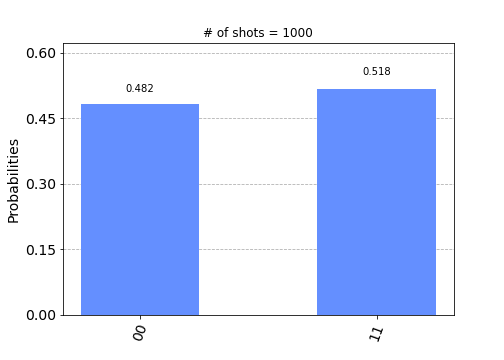
\includegraphics[height=0.4\textheight]{figures/itercomp/qca1.png}\hspace{0.5cm}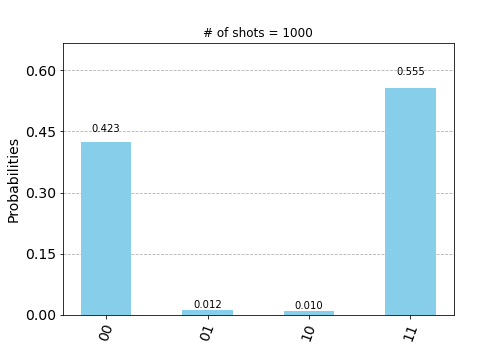
\includegraphics[height=0.4\textheight]{figures/itercomp/rqca1.png}\end{center}{\tiny Measurement statistics of a Bell state: noise-free simulation (left) and \texttt{ibmq\_santiago} (right). The outcomes $01$ and $10$ appear with non-zero frequency independently of the number of shots: the estimator is biased.}}
\ona{\begin{figure}[htb]\centering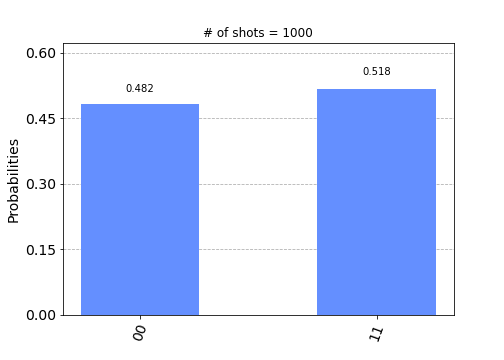
\includegraphics[width=0.42\linewidth]{figures/itercomp/qca1.png}\hfill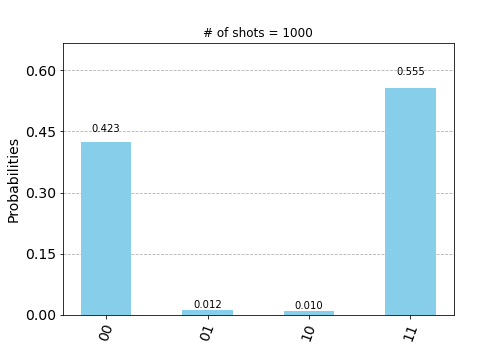
\includegraphics[width=0.42\linewidth]{figures/itercomp/rqca1.png}\caption{Measurement statistics of a Bell state prepared by a Hadamard and a CNOT: noise-free simulation (left) and IBM's five-qubit device \texttt{ibmq\_santiago} (right) \cite{kungurtsev2022iteration}. The outcomes $01$ and $10$ appear with non-zero frequency independently of the number of shots, so the sample mean of any observable is biased.}\label{fig:ch06:bell}\end{figure}}
\end{frame}

\begin{frame}\ft{The noise model}
\ona{Write a function evaluation as}
\begin{equation}\label{eq:ch06:feval}
    f' \sim F(\boldsymbol\theta,\xi) = f(\boldsymbol\theta) + n(\boldsymbol\theta,\xi),
\end{equation}
\ona{where $f = C$ is the true objective and $\xi$ the randomness of the device. Two assumptions:}
\begin{itemize}\setlength\itemsep{0.3em}
    \item[\textbf{A1}] (bounded bias) $n(\boldsymbol\theta_k,\xi_k) = r_k + b_k$ with $\mathbb E[r_k] = 0$, $\mathbb E\|r_k\|^2 \le \sigma^2$, and $\|b_k\| \le b$ almost surely.
    \item[\textbf{A2}] (smoothness) $\nabla F(\cdot,\xi)$ is $L$-Lipschitz for all $\xi$.
\end{itemize}
\ona{Both are natural for VQAs: a gate error $H_i \mapsto \tilde H_i$ perturbs \eqref{eq:ch06:cost} by at most $b = 2\|e^{i\theta H} - e^{i\theta\tilde H}\|\,\sigma^M(O)$, where $\sigma^M(O)$ is the largest eigenvalue of $O$, since all other factors are norm-preserving; and $C$ is a trigonometric polynomial with Hessian bounded by $L = \sigma^M(O)$ in the ideal case. Shot noise contributes to $\sigma^2$ and shrinks with the number of shots; the bias $b$ does not.}
\onp{Gate errors give $b \le 2\|e^{i\theta H}-e^{i\theta\tilde H}\|\,\sigma^M(O)$; smoothness $L = \sigma^M(O)$; more shots shrink $\sigma^2$ but not $b$.}
\end{frame}

\section{The estimators, recalled}

\begin{frame}\ft{Three ways to a gradient}
\ona{Recall from \Chap~\chref{C.PSR}: the parameter-shift rule gives an exact gradient from $2L$ shifted evaluations, $\partial_jC = [C(\boldsymbol\theta + \tfrac\pi2e_j) - C(\boldsymbol\theta - \tfrac\pi2e_j)]/2$; the derivative-free estimators use two evaluations along a random direction $\boldsymbol\Delta_k$ with perturbation $c_k$:}
\begin{align}
    \text{SPSA:}\quad & [\boldsymbol g_k]_i \sim \frac{F(\boldsymbol\theta_k + c_k\boldsymbol\Delta_k,\xi_k^1) - F(\boldsymbol\theta_k - c_k\boldsymbol\Delta_k,\xi_k^2)}{2c_k[\boldsymbol\Delta_k]_i}, \label{eq:ch06:spsa}\\
    \text{two-point (2PFA):}\quad & \boldsymbol g_k \sim \frac{F(\boldsymbol\theta_k + c_k\boldsymbol\Delta_k,\xi_k^1) - F(\boldsymbol\theta_k,\xi_k^2)}{c_k}\,\boldsymbol\Delta_k, \label{eq:ch06:2pfa}
\end{align}
\ona{each followed by $\boldsymbol\theta_{k+1} = \boldsymbol\theta_k - \alpha_k\boldsymbol g_k$. The two-point estimator is an unbiased gradient of the Gaussian smoothing $f_c(\boldsymbol\theta) = \mathbb E_{\boldsymbol\Delta}f(\boldsymbol\theta + c\boldsymbol\Delta)$, with $|f_c - f| \le \tfrac{c^2}{2}Lp$ and $\|\nabla f_c - \nabla f\| \le \tfrac c2L(p+3)^{3/2}$; these smoothing bounds \eqref{eq:ch06:smooth} enter the theorems below.}
\begin{equation}\label{eq:ch06:smooth}
    f_c(\boldsymbol\theta) = \mathbb E_{\boldsymbol\Delta\sim\mathcal N(0,\one)} f(\boldsymbol\theta + c\boldsymbol\Delta).
\end{equation}
\ona{Existing guarantees assume unbiased evaluations \cite{ghadimi2013stochastic} or strong convexity \cite{granichin2014simultaneous}, neither of which holds for VQAs.}
\end{frame}

\section{Iteration complexity with bias}

\begin{frame}\ft{Two-point approximation with bias}
\onp{\footnotesize}
\begin{thm}[\citet{kungurtsev2022iteration}]\label{thm:ch06:twopoint}
Under A1--A2, consider the two-point approximation \eqref{eq:ch06:2pfa} with $K$ iterations and constant step $\alpha_k \equiv \alpha/\sqrt K$, $\alpha \le L/4$. Then
\begin{equation}\label{eq:ch06:tp}
    \min_{k\le K}\mathbb E\|\nabla f(\boldsymbol\theta_k)\|^2 \le
    \underbrace{\frac{4(f_c(\boldsymbol\theta_0) - f_c^*)}{\alpha\sqrt K}}_{\text{optimization}}
    + \underbrace{\frac{2L\alpha(\sigma^2 + 8b^2/c^2)}{\alpha\sqrt K}}_{\text{noise and bias}}
    + \underbrace{\Big[\frac{2b^2}{c^2} + \frac{c^2}{2}L(p+3)^3\Big]}_{\text{effect of bias}}.
\end{equation}
With diminishing steps $\alpha_k = \alpha/k^\gamma$, $\gamma \in (1/2,1]$, and a random iterate $\boldsymbol\theta_R$ drawn with probability $\propto \alpha_k$, the same bound holds with $\sqrt K$ replaced by $K^\gamma$.
\end{thm}
\begin{itemize}\setlength\itemsep{0.2em}
    \item The first two terms vanish as $K \to \infty$ at the rate $1/\sqrt K$ of unbiased stochastic gradient descent; the bias enlarges the constant.
    \item The third term does not vanish: no number of iterations brings the gradient norm below it. Minimising it over the perturbation size gives $c^* = [4b^2/(L(p+3)^3)]^{1/4}$\ona{, see Fig.~\ref{fig:ch06:cstar}}.
\end{itemize}
\end{frame}

\begin{frame}\ft{The optimal perturbation}
\figslide[height=0.55\textheight]{figures/itercomp/cstar.pdf}{Logarithm of the optimal perturbation $c^*$ of the two-point approximation as a function of the bias $b$ and the number of parameters $p$ \cite{kungurtsev2022iteration}: more bias calls for coarser perturbations, more parameters for finer ones.}{fig:ch06:cstar}
\end{frame}

\begin{frame}\ft{SPSA with bias}
\ona{For SPSA one uses Spall's lemma: without bias in the evaluations, the estimate \eqref{eq:ch06:spsa} satisfies $\boldsymbol g_k - \nabla f(\boldsymbol\theta_k) = \boldsymbol r_k + \boldsymbol b_0(\boldsymbol\theta_k)$ with $\mathbb E\boldsymbol r_k = 0$ and $\|\boldsymbol b_0\| \le b_0 c_k^2$, provided $\boldsymbol\Delta_k$ is symmetric with bounded components and inverse moments. Add the assumption that $[\boldsymbol\Delta_k]_i^{-1} \le B_3$ almost surely.}
\begin{thm}[\citet{kungurtsev2022iteration}]\label{thm:ch06:spsa}
Under A1--A2 and the SPSA conditions above, with $K$ iterations and $\alpha_k \equiv \alpha/\sqrt K$, $\alpha \le L/2$,
\begin{equation}\label{eq:ch06:spsabound}
    \min_{k\le K}\mathbb E\|\nabla f(\boldsymbol\theta_k)\|^2 \le
    \frac{4(f_c(\boldsymbol\theta_0)-f_c^*)}{\alpha\sqrt K}
    + \frac{2L\alpha\big[\frac{\sigma^2B_3^2}{c_k^2} + 2b_0c_k^2 + \frac{2b^2B_3^2}{c_k^2}\big]}{\sqrt K}
    + \Big[b_0c_k^2 + \frac{b^2B_3^2}{c_k^2}\Big],
\end{equation}
and analogously for diminishing steps.
\end{thm}
\ona{The structure is the same: an optimization term, a noise-and-bias term, both decaying, and an asymptotic bias floor. Unlike the two-point method, the dimension $p$ enters SPSA only through $b_0$, and the user controls two knobs, $c_k$ and $B_3$, to mitigate the bias.}
\end{frame}

\begin{frame}\ft{The bound surface for SPSA}
\figslide[height=0.55\textheight]{figures/itercomp/exp.pdf}{The right-hand side of \eqref{eq:ch06:spsabound} for $L = 8$, $\alpha = 4$, $\sigma = 1$, $K = 10^5$, as a function of bias $b$ and perturbation $c$, logarithmic scale \cite{kungurtsev2022iteration}. For each bias there is an optimal perturbation size.}{fig:ch06:exp}
\end{frame}

\begin{frame}\ft{Parameter-shift rule with bias}
\ona{Without bias, the parameter-shift rule is an exact gradient, so with shot noise it is an unbiased stochastic gradient; the device bias then puts us exactly in the setting of biased stochastic gradient descent \cite{ajalloeian2020convergence}, with bias bounded by $\zeta^2 = b$ and no gradient-proportional terms. Hence, for constant step $\alpha \le 1/L$,}
\begin{equation}\label{eq:ch06:psrbound}
    \frac1K\sum_{k=1}^K\|\nabla f(\boldsymbol\theta_k)\|^2 \le \frac{2F}{K\alpha} + \alpha L\sigma^2 + b,
\end{equation}
\ona{where $F$ is the initial optimality gap.}
\textbf{Comparison of \eqref{eq:ch06:tp}, \eqref{eq:ch06:spsabound}, \eqref{eq:ch06:psrbound}.}
\begin{enumerate}\setlength\itemsep{0.1em}
    \item All three have the same rate; the bias affects constants and the floor, not the rate.
    \item The error grows at least with the square of $\sigma^M(O)$, through $L$ and $b$.
    \item PSR has the smallest bias floor and constants, as an exact gradient should; but it costs $2p$ evaluations per iteration.
    \item SPSA is the most tuneable: $B_3$ and $c_k$ are the user's, and aggressive choices mitigate bias; $p$ enters only via $b_0$.
    \item The two-point approximation is the option of last resort: one knob, and a floor scaling with $(p+3)^3$.
    \item More shots reduce $\sigma^2$, improving both the rate and the floor; the floor's dependence on $b$ remains.
\end{enumerate}
\end{frame}

\section{Numerical experiments}

\begin{frame}\ft{Set-up: MaxCut on a 4-regular graph}
\ona{The test case is depth-one QAOA for MaxCut on a four-vertex instance, Fig.~\ref{fig:ch06:qaoa}, simulated with Qiskit Aer with a custom noise model: depolarising channels of strength $10^{-3}$ per single-qubit gate and $10^{-2}$ per CNOT, and a read-out assignment matrix $P$. Two read-out models are used: a random sparse row-stochastic $P_{\rm rand}$, and a realistic single-bit-flip model built from the published assignment probabilities $p(1|0)$, $p(0|1)$ of IBM devices (\texttt{armonk}, \texttt{lima}, \texttt{bogota}, \dots), whose asymmetry $\tilde b = |p(0|1) - p(1|0)|$ ranges from $0.004$ to $0.14$.}
\figslide[height=0.35\textheight]{figures/itercomp/qaoa4.pdf}{The QAOA circuit for 4 qubits; one layer is marked, and dots denote its repetition to the desired depth \cite{kungurtsev2022iteration}.}{fig:ch06:qaoa}
\end{frame}

\begin{frame}\ft{SPSA under biased read-out}
\figslide[height=0.55\textheight]{figures/itercomp/spsa_comb.png}{Noisy objective values along SPSA iterations for four values of the estimated bias $\hat b$, perturbation $c = 0.01$ \cite{kungurtsev2022iteration}. The bias is estimated by fitting a mixture of a normal and a uniform distribution to the empirical distribution of objective values. In line with Theorem~\ref{thm:ch06:spsa}, the iteration complexity grows with the bias.}{fig:ch06:spsacomb}
\end{frame}

\begin{frame}\ft{SPSA on the noise models of three IBM devices}
\onp{\begin{center}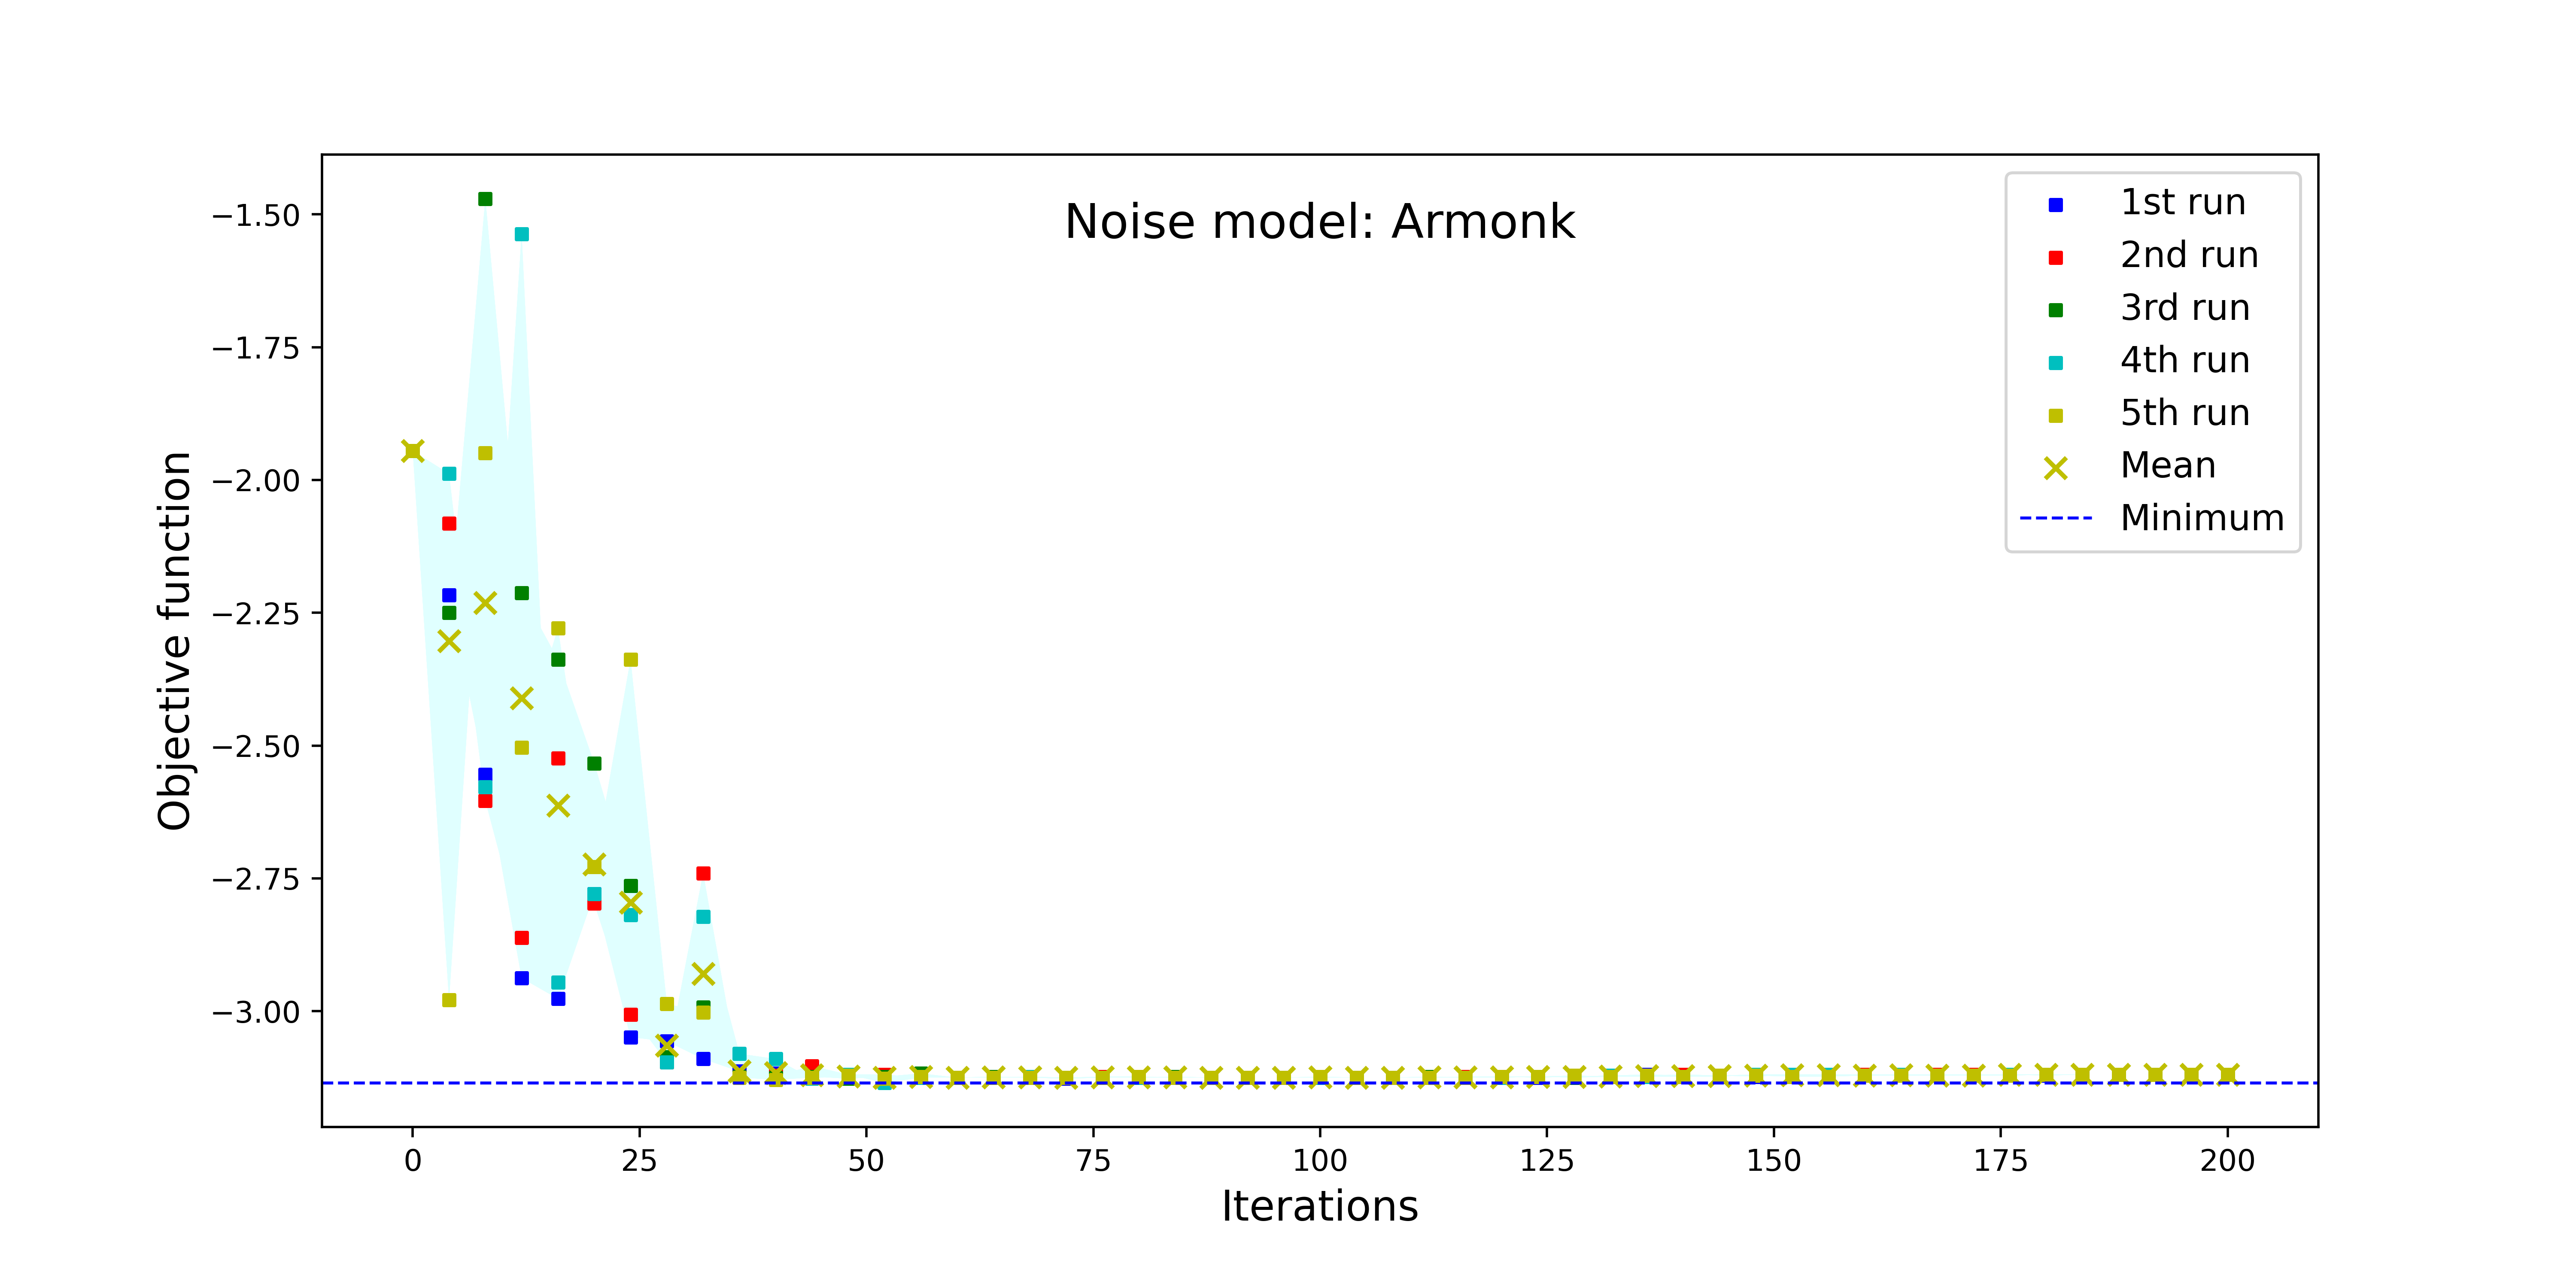
\includegraphics[width=0.32\linewidth]{figures/itercomp/spsa_arm.png}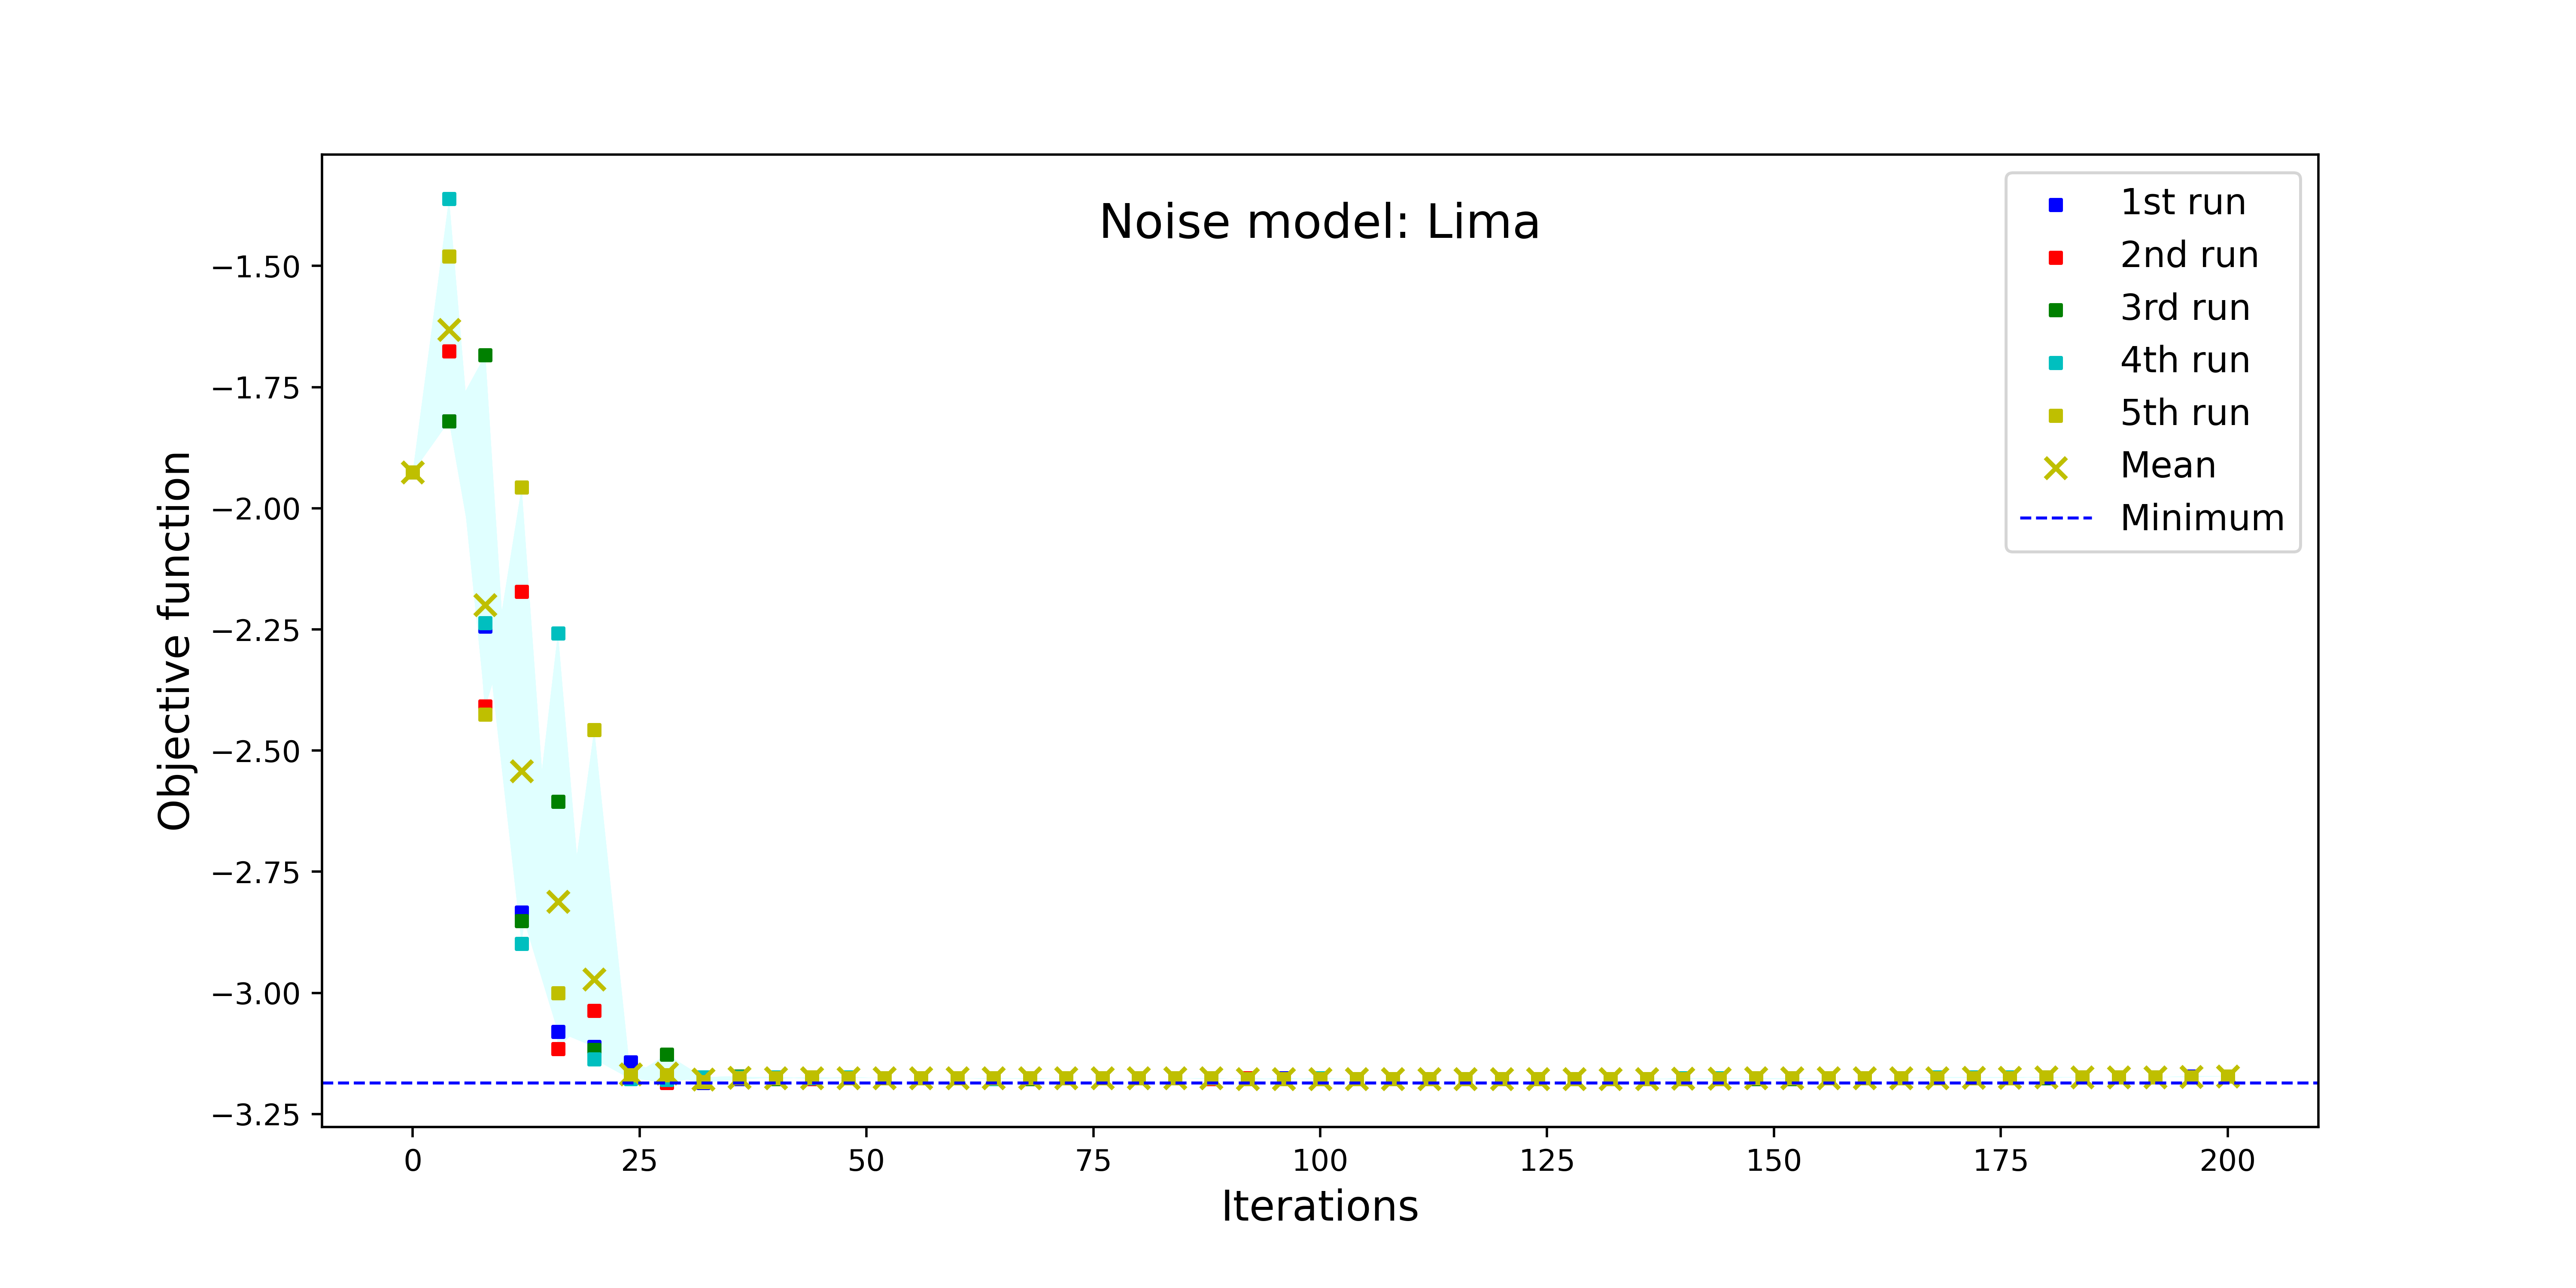
\includegraphics[width=0.32\linewidth]{figures/itercomp/spsa_lima.png}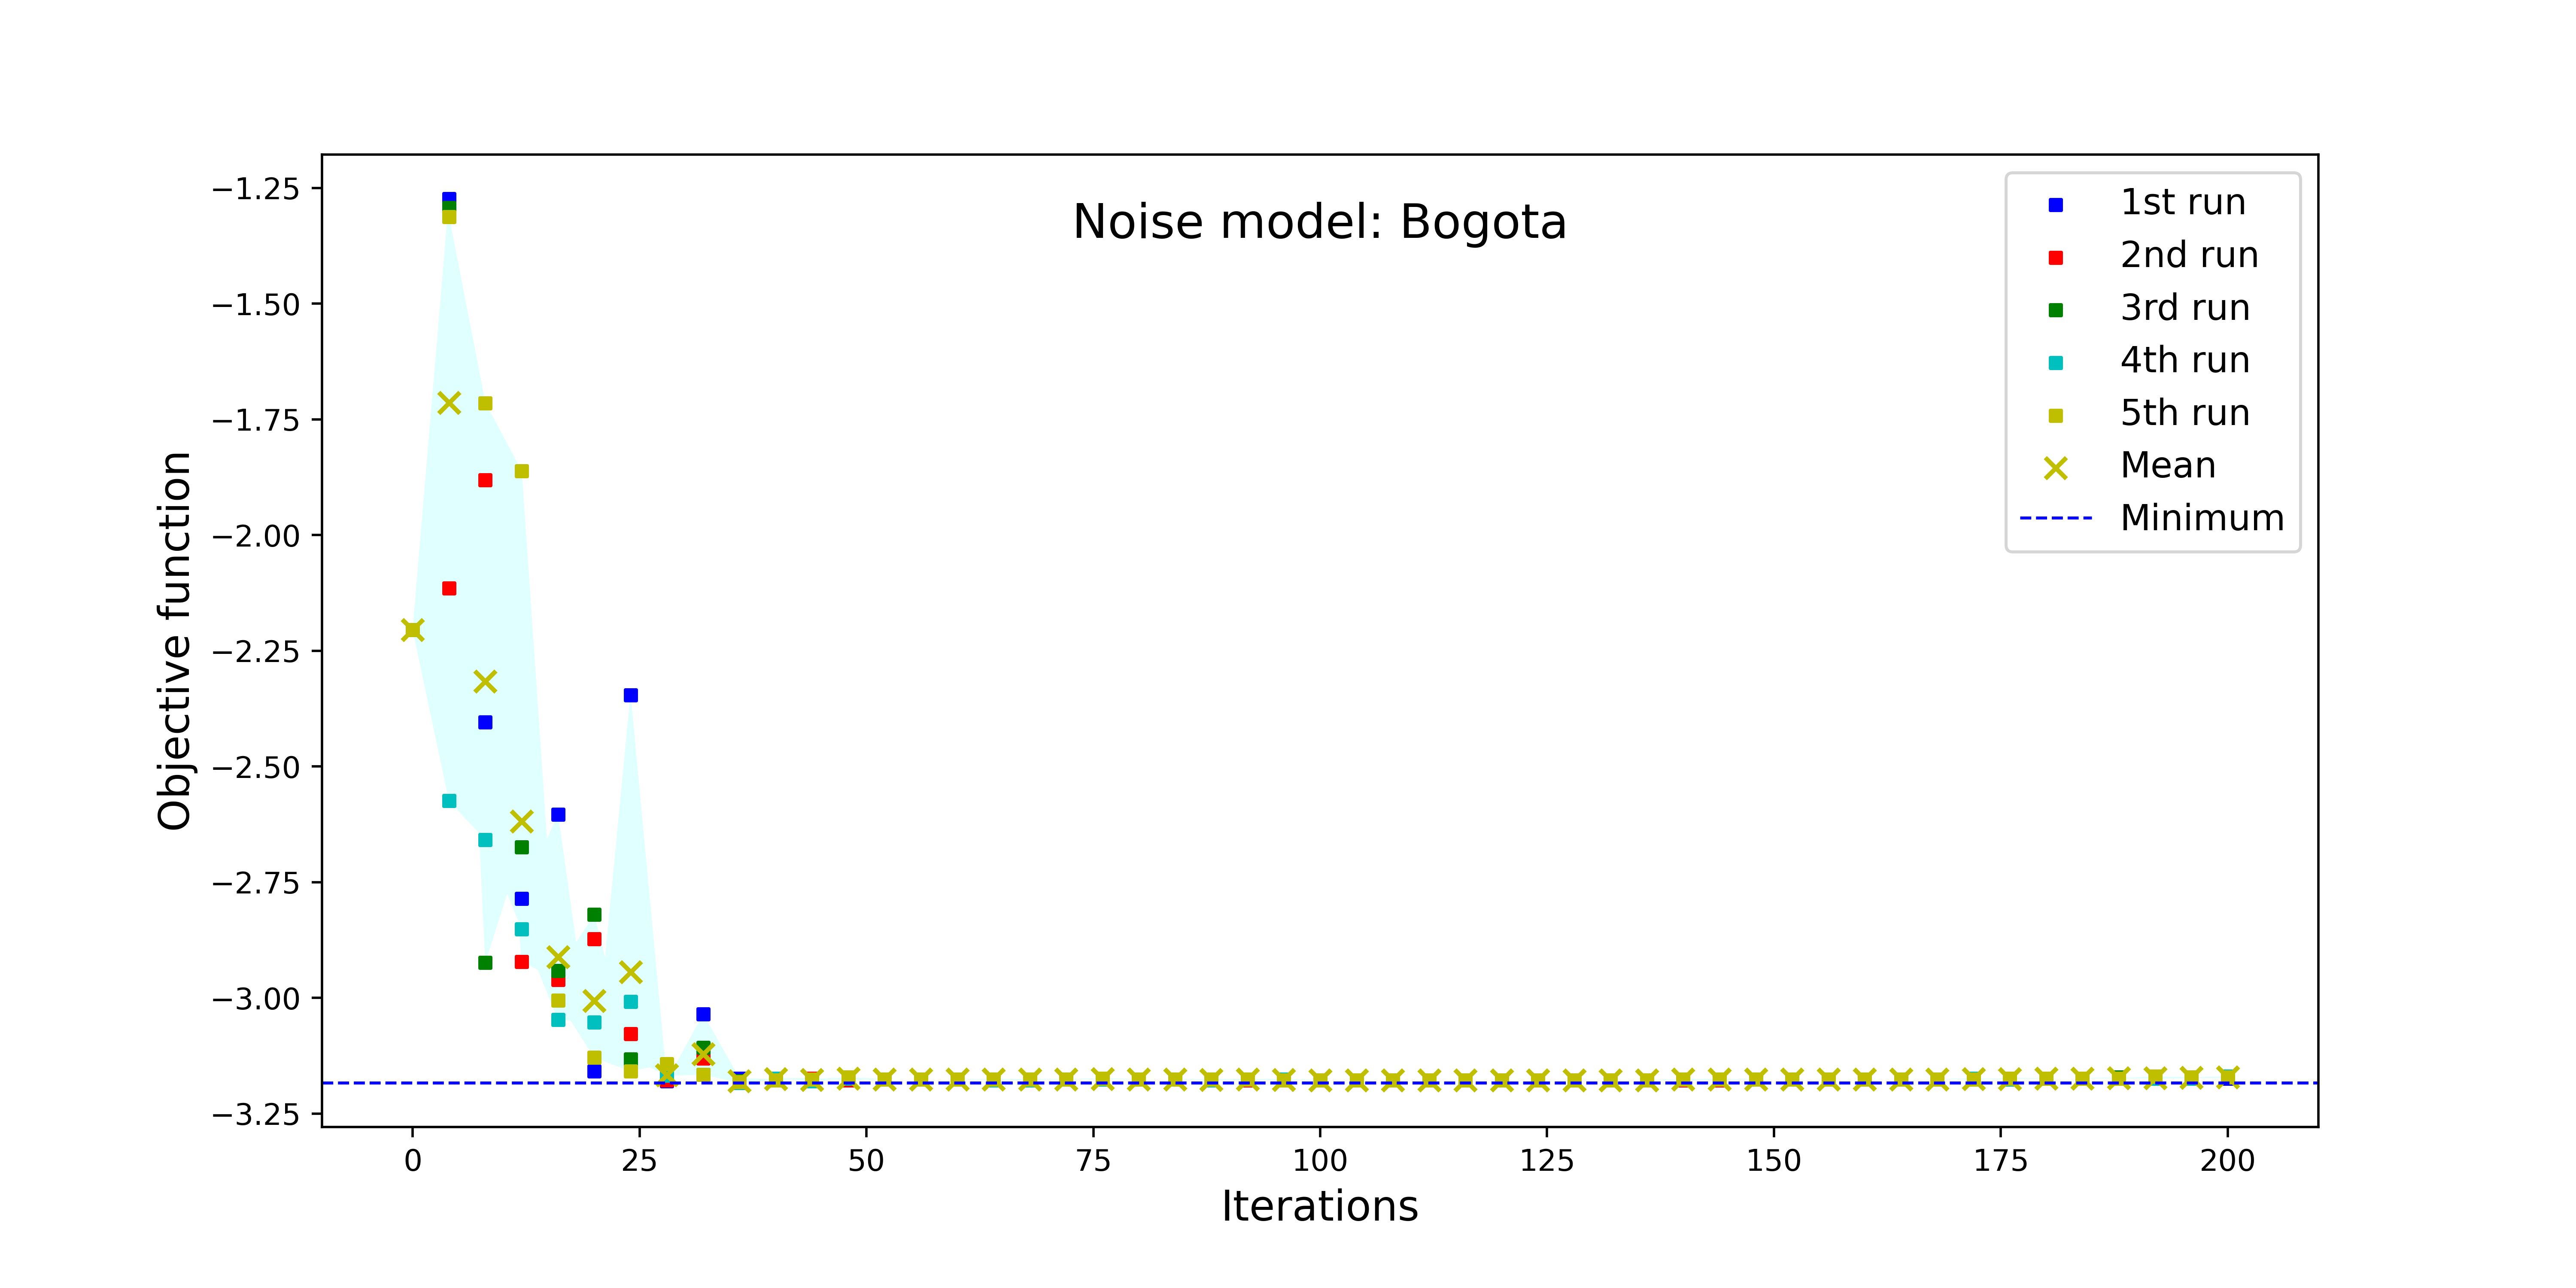
\includegraphics[width=0.32\linewidth]{figures/itercomp/spsa_bog.png}\end{center}{\tiny Five SPSA runs each, mean (crosses) and one standard deviation (shaded), with the read-out models of \texttt{armonk}, \texttt{lima}, and \texttt{bogota}.}}
\ona{\begin{figure}[htb]\centering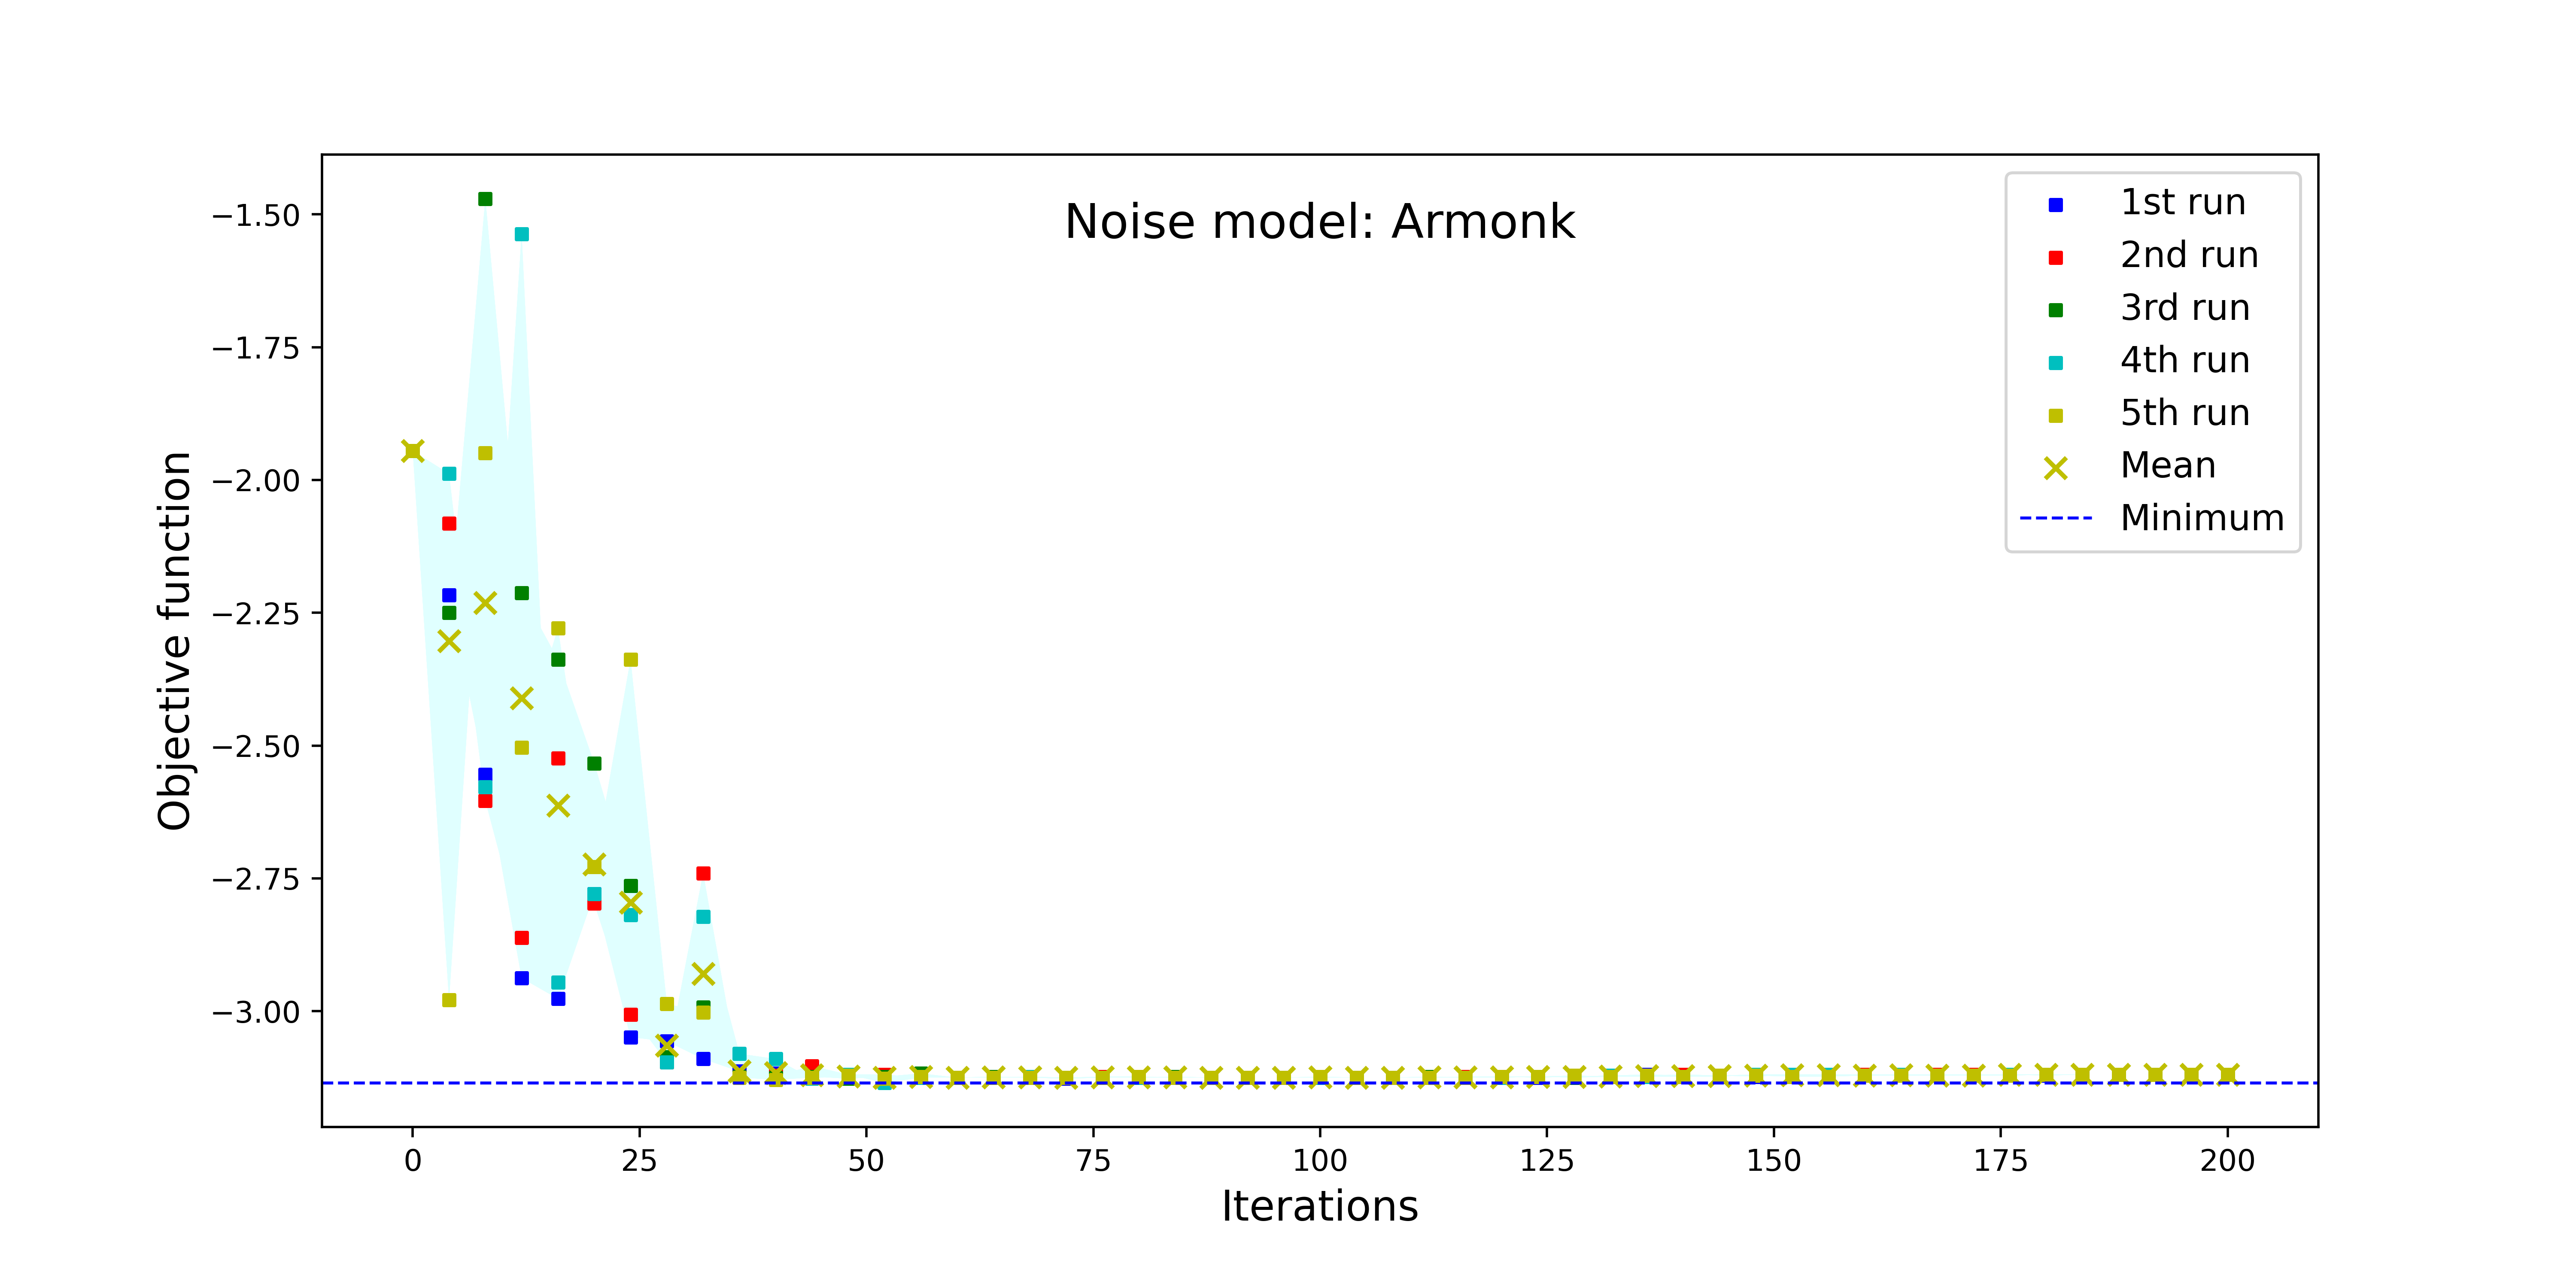
\includegraphics[width=0.32\linewidth]{figures/itercomp/spsa_arm.png}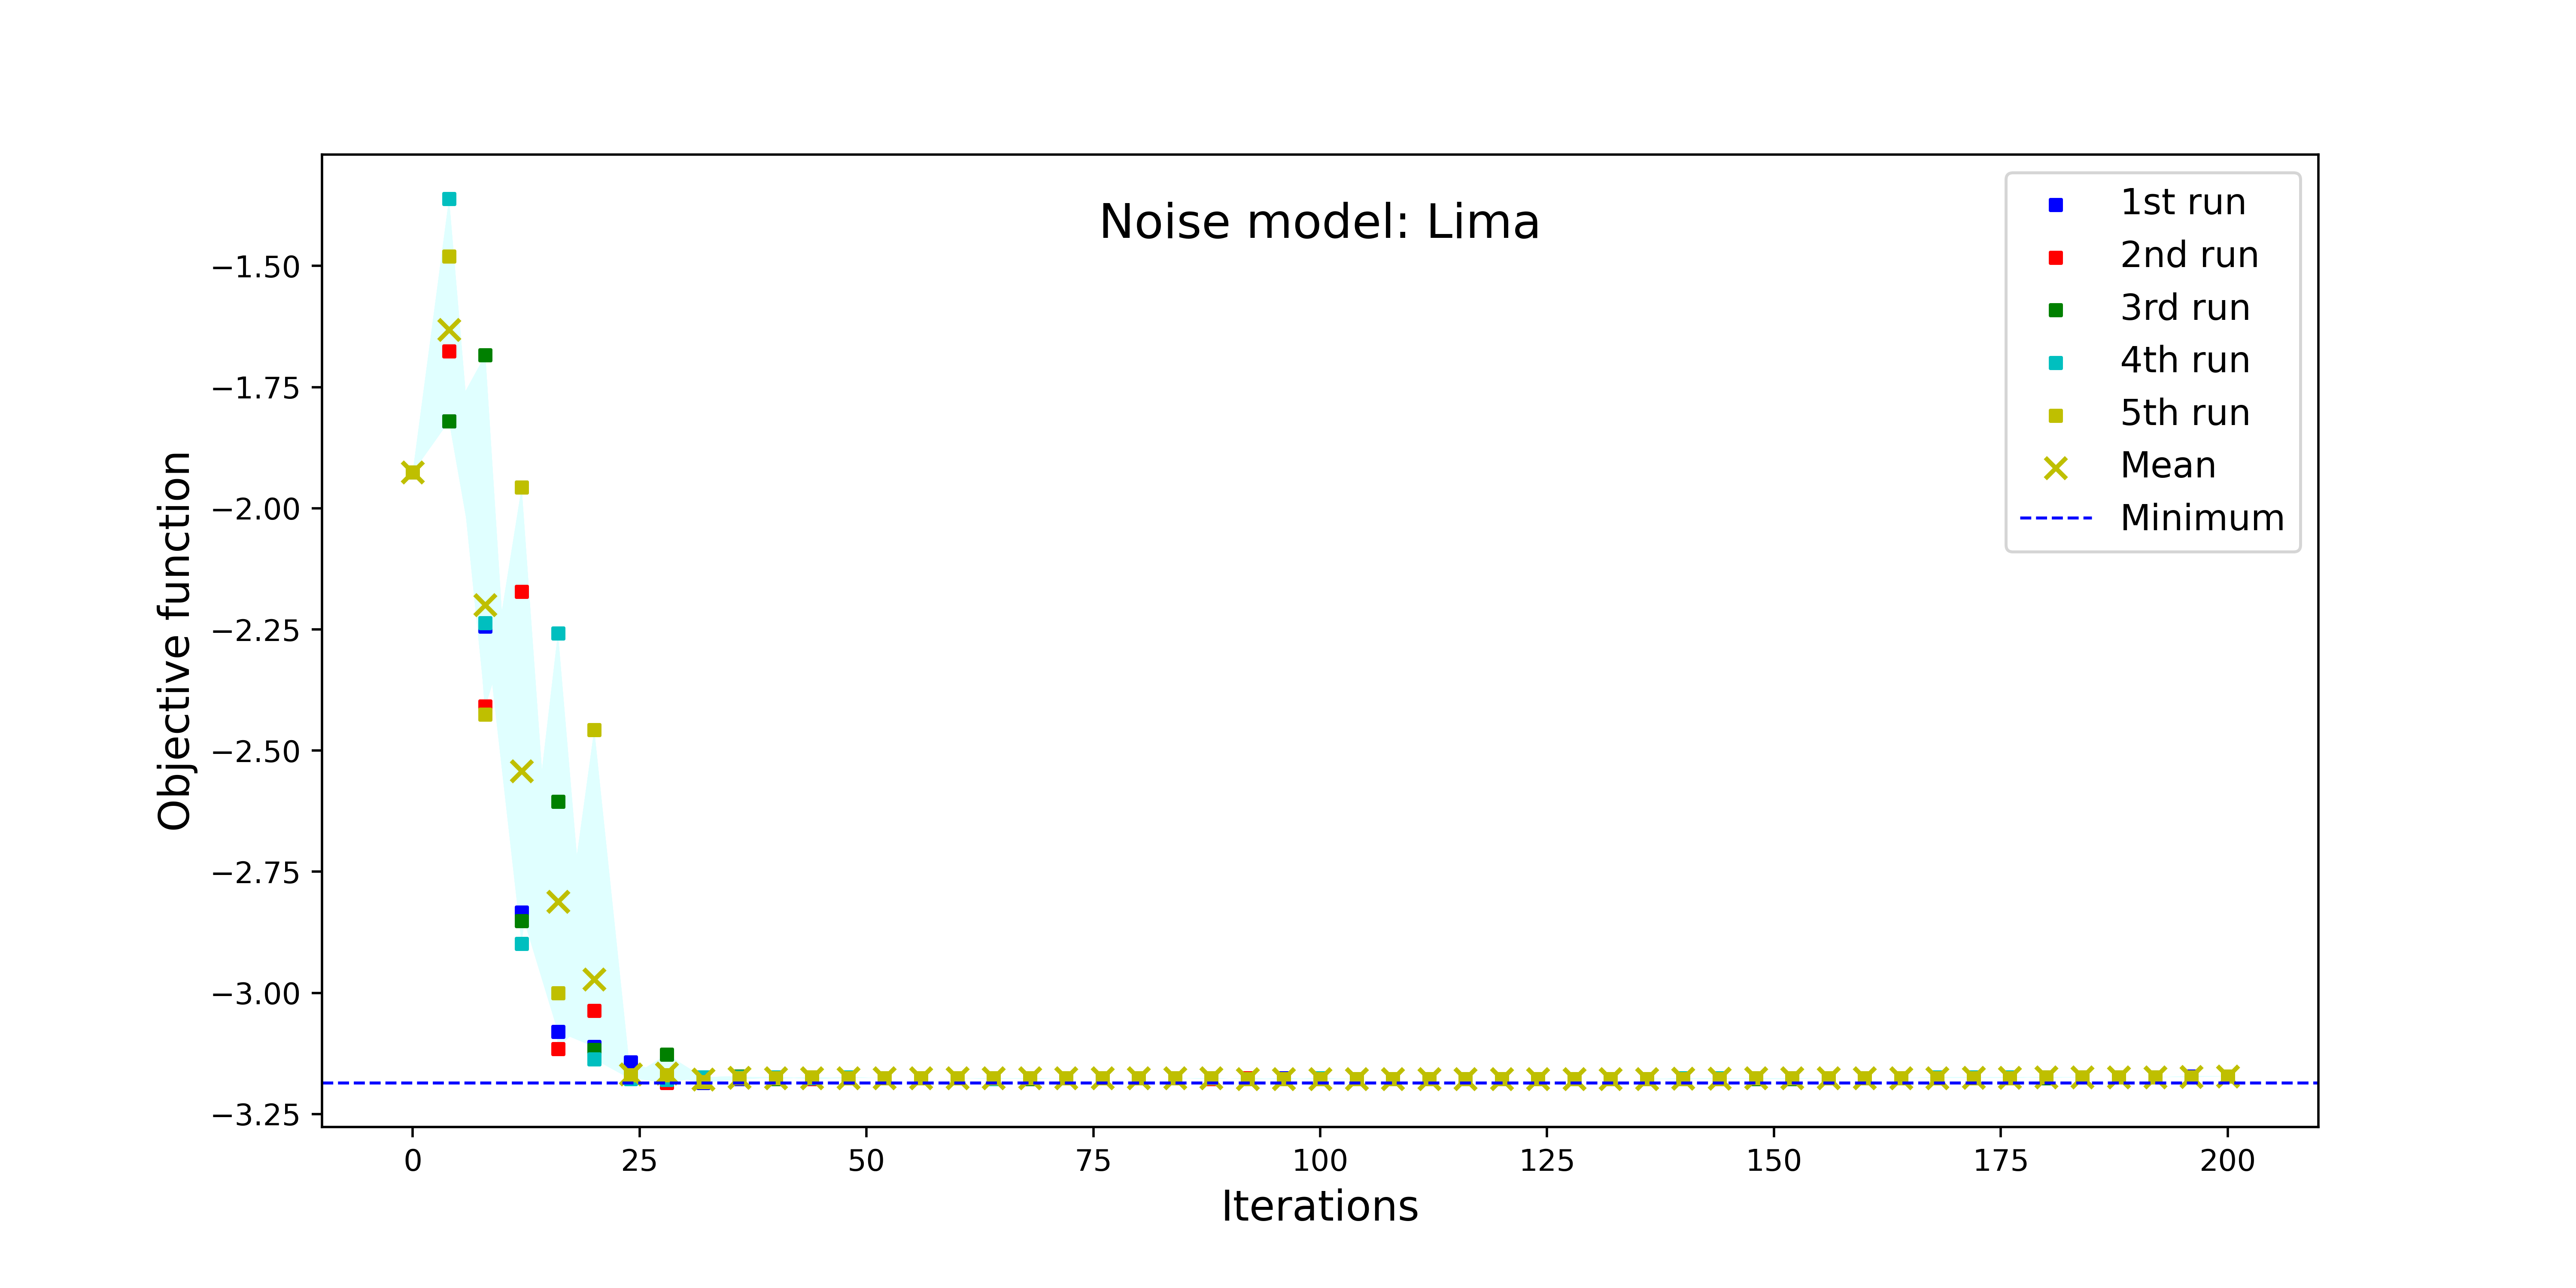
\includegraphics[width=0.32\linewidth]{figures/itercomp/spsa_lima.png}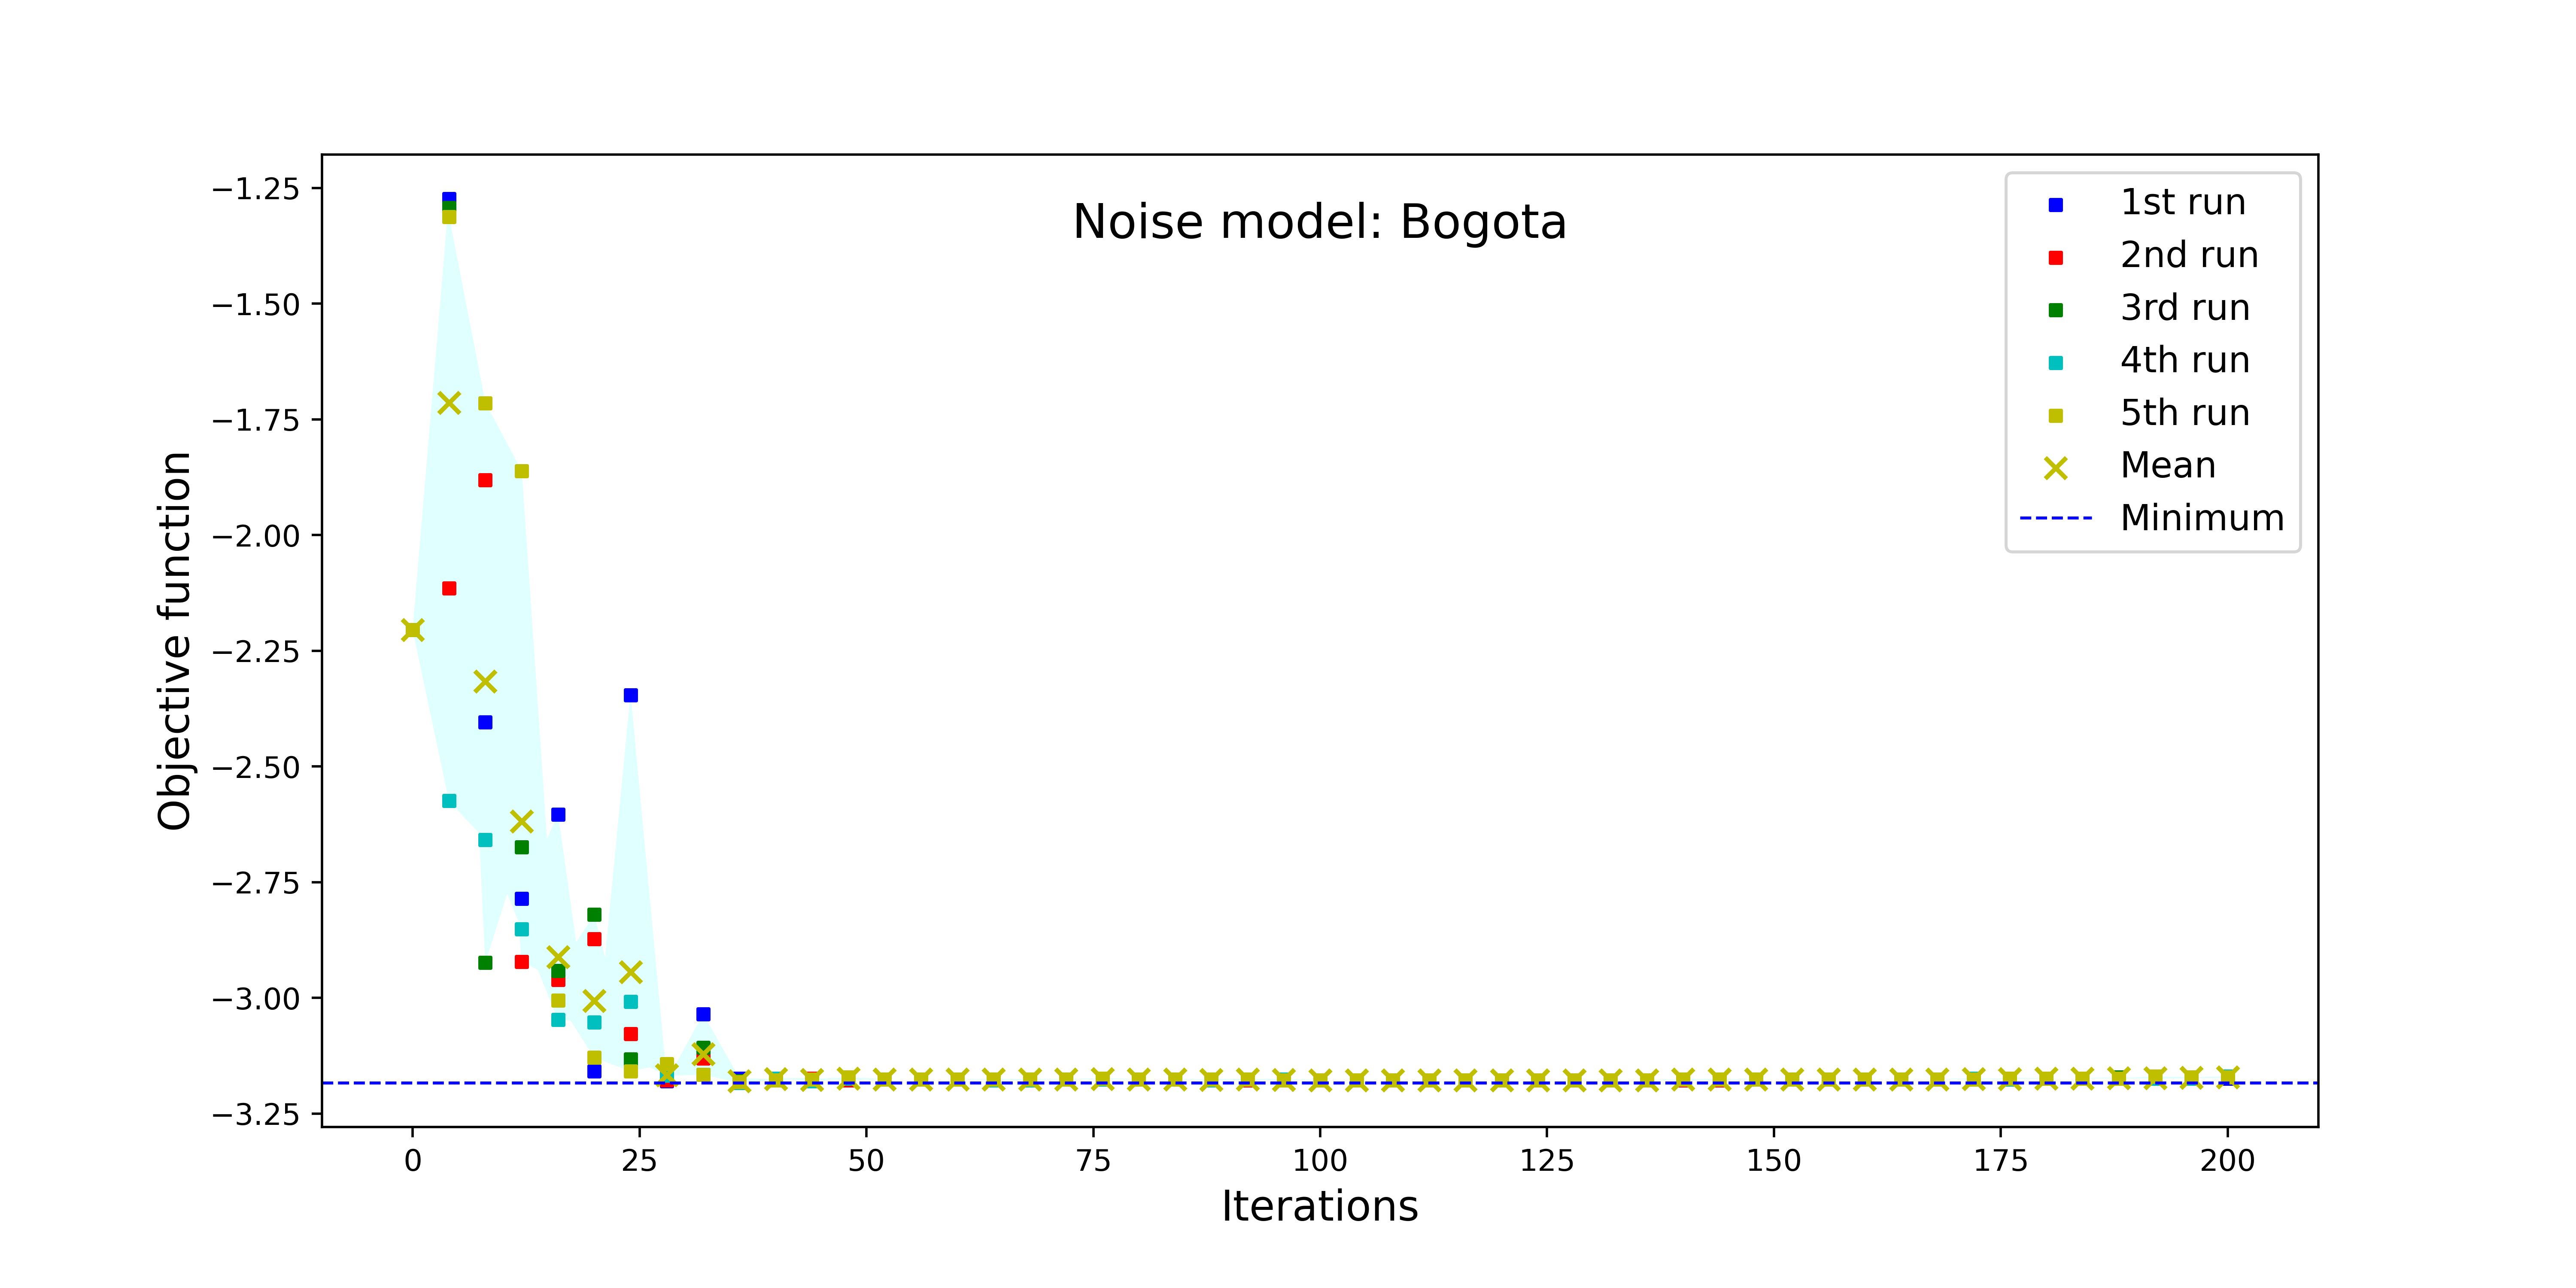
\includegraphics[width=0.32\linewidth]{figures/itercomp/spsa_bog.png}\caption{Objective values of five SPSA runs, their mean (crosses) and one standard deviation (shaded), under the read-out noise models of \texttt{ibmq\_armonk}, \texttt{ibmq\_lima}, and \texttt{ibmq\_bogota} \cite{kungurtsev2022iteration}. The device with the largest read-out asymmetry, \texttt{bogota}, converges to the highest noise-dominated level.}\label{fig:ch06:devices}\end{figure}}
\end{frame}

\begin{frame}\ft{SPSA versus two-point versus parameter shift}
\ona{Finally, the three estimators are compared from ten random starting points with step sizes $\alpha$ and perturbations $c$ in $\{10^{-1},10^{-2},10^{-3}\}$, under the \texttt{lima} noise model. Two representative regimes:}
\onp{\begin{center}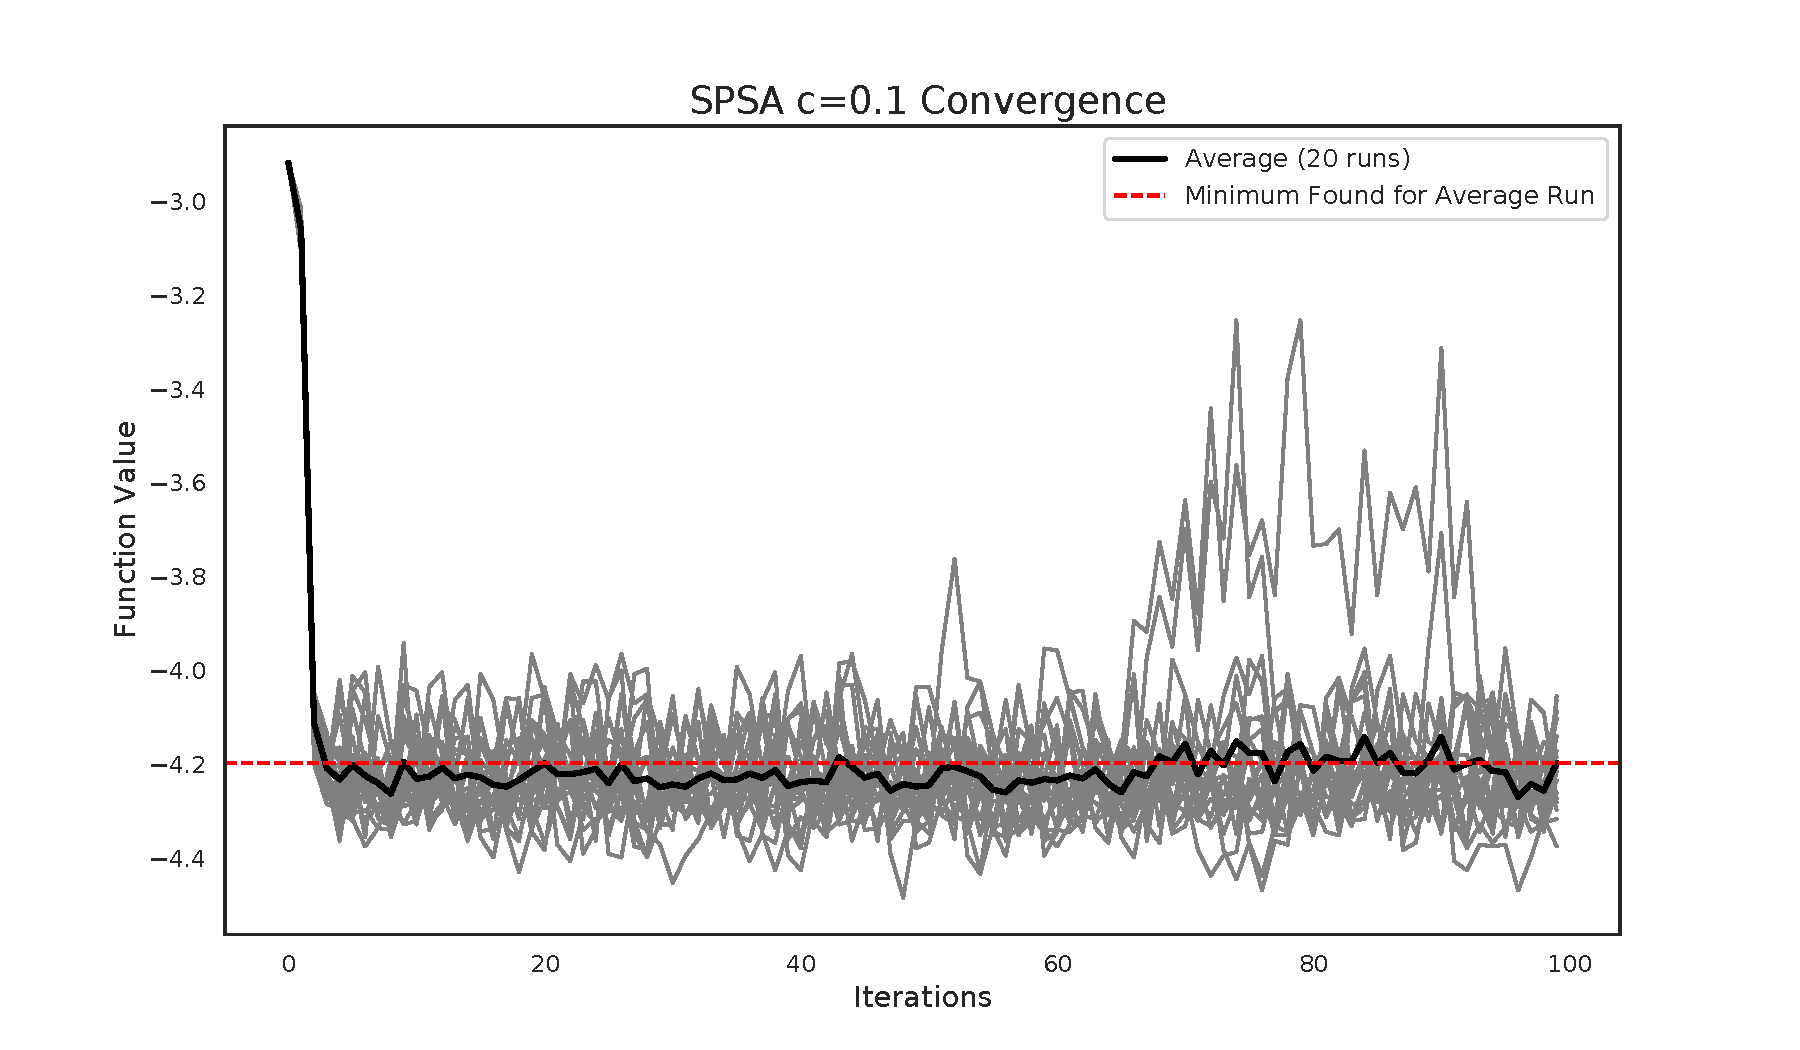
\includegraphics[width=0.32\linewidth]{figures/itercomp/cmp_spsa_c01_a01.pdf}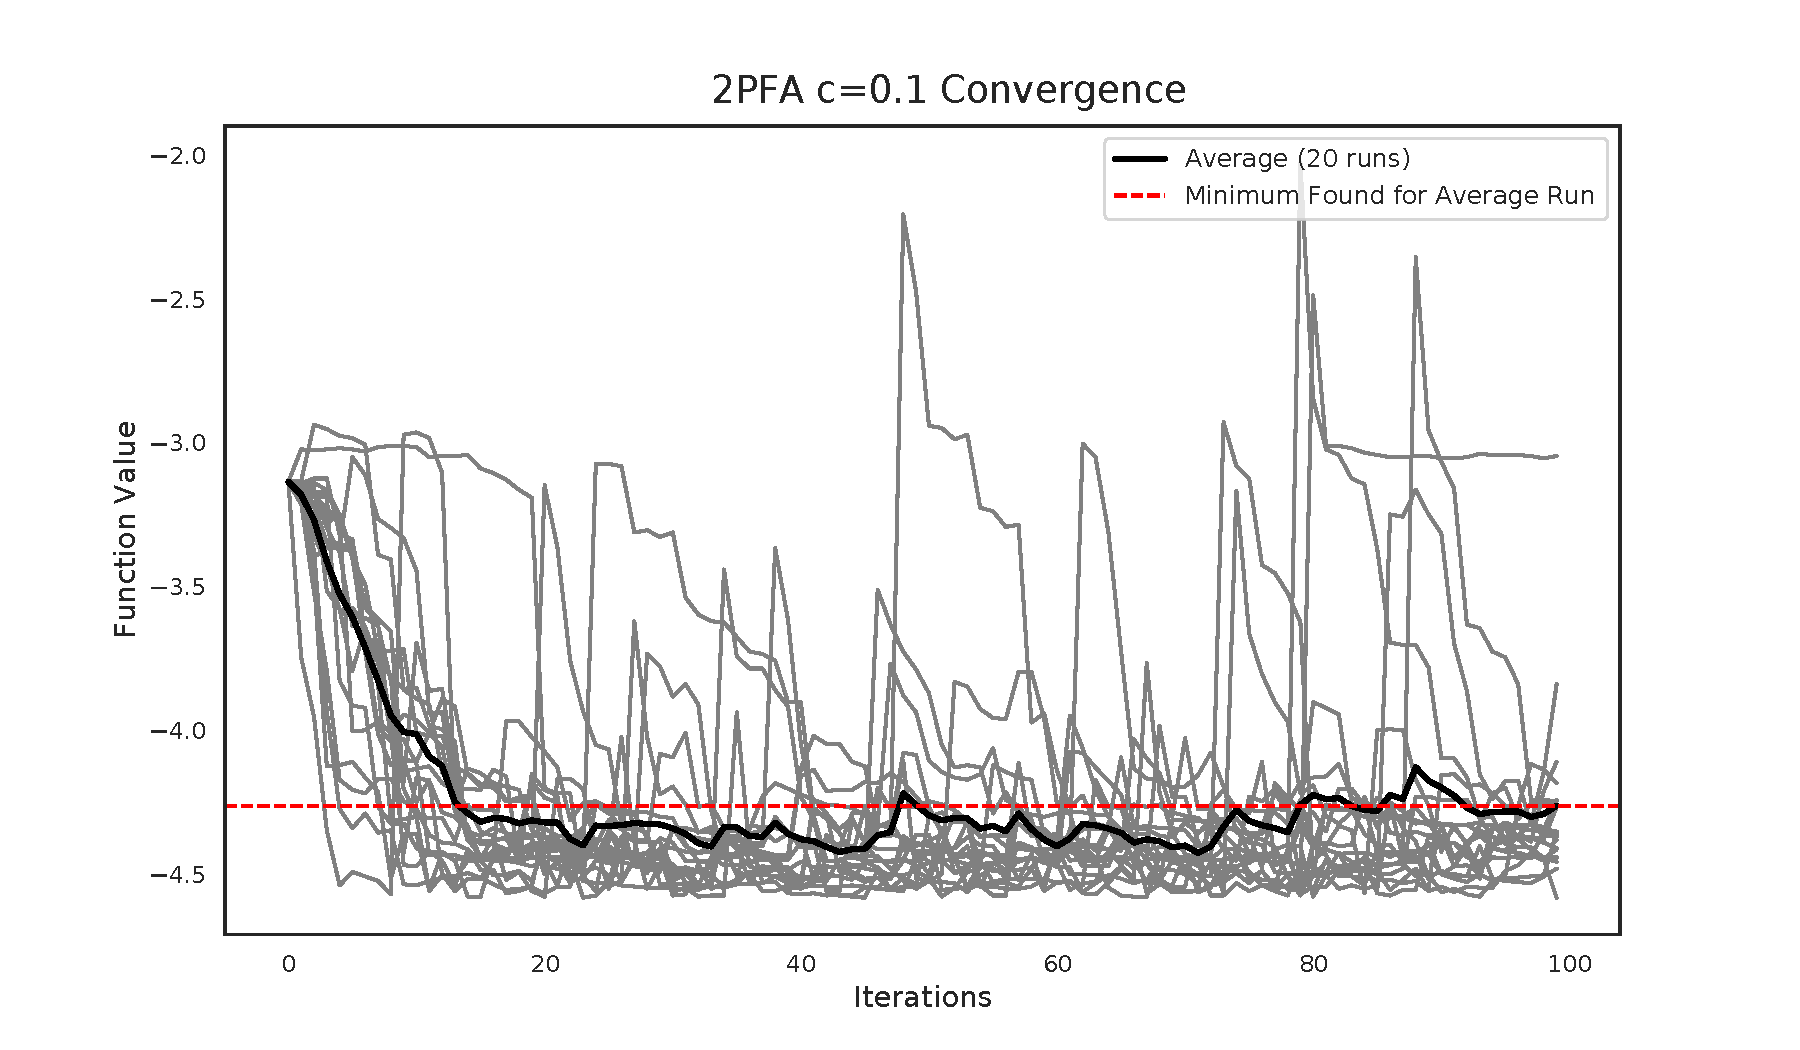
\includegraphics[width=0.32\linewidth]{figures/itercomp/cmp_2pfa_c01_a01.pdf}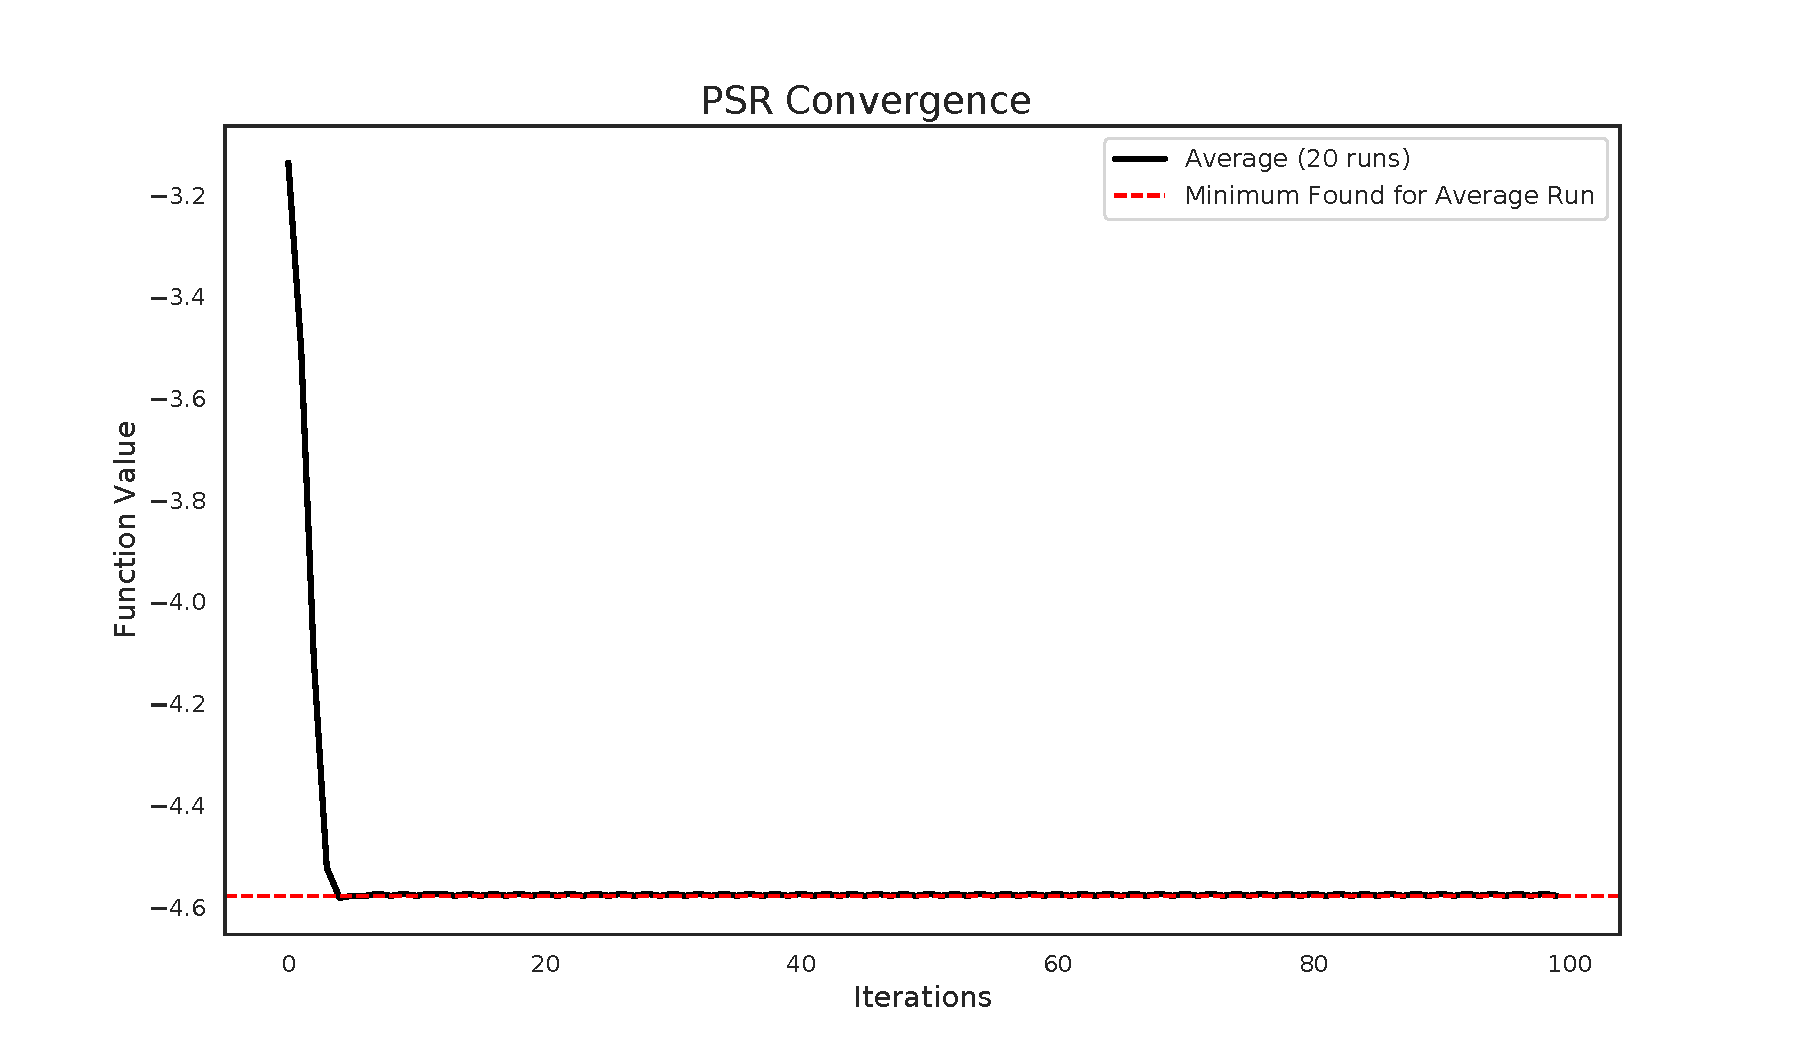
\includegraphics[width=0.32\linewidth]{figures/itercomp/cmp_psr_a01.pdf}\end{center}{\tiny Large step $\alpha = 0.1$, large perturbation $c = 0.1$: SPSA (left), two-point (centre), parameter shift (right).}}
\ona{\begin{figure}[htb]\centering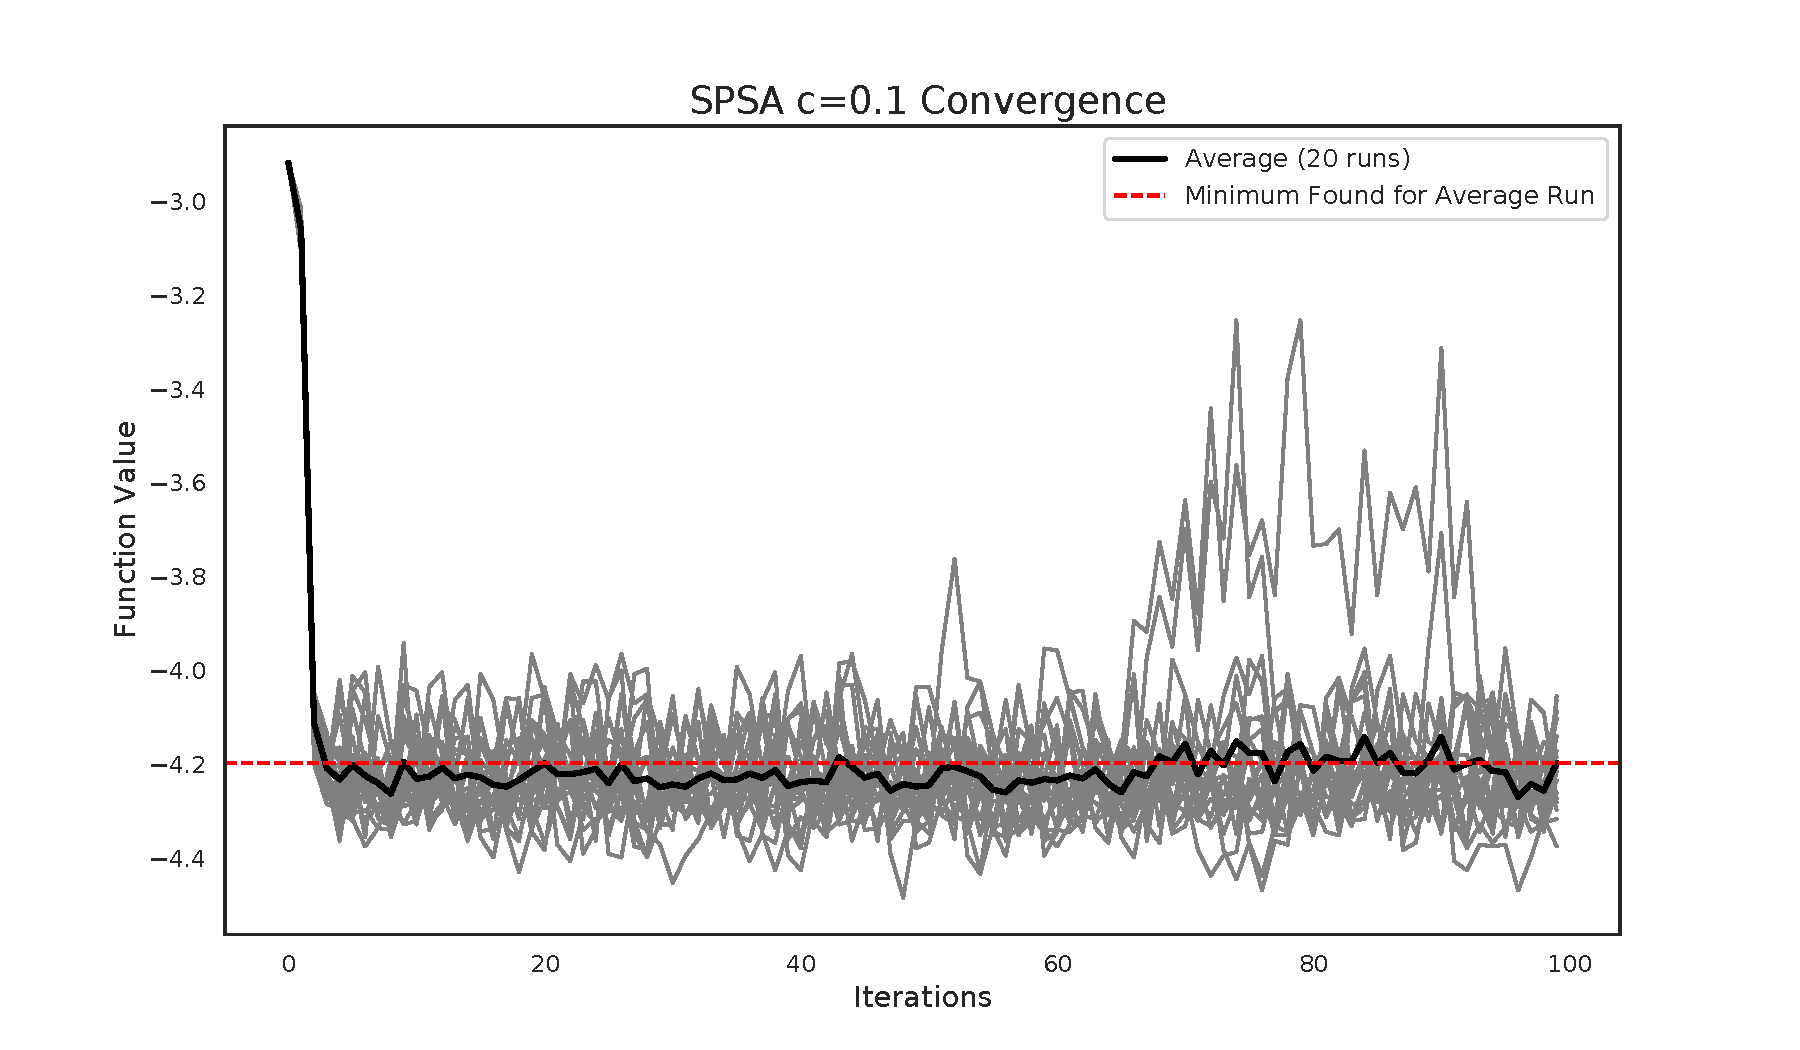
\includegraphics[width=0.32\linewidth]{figures/itercomp/cmp_spsa_c01_a01.pdf}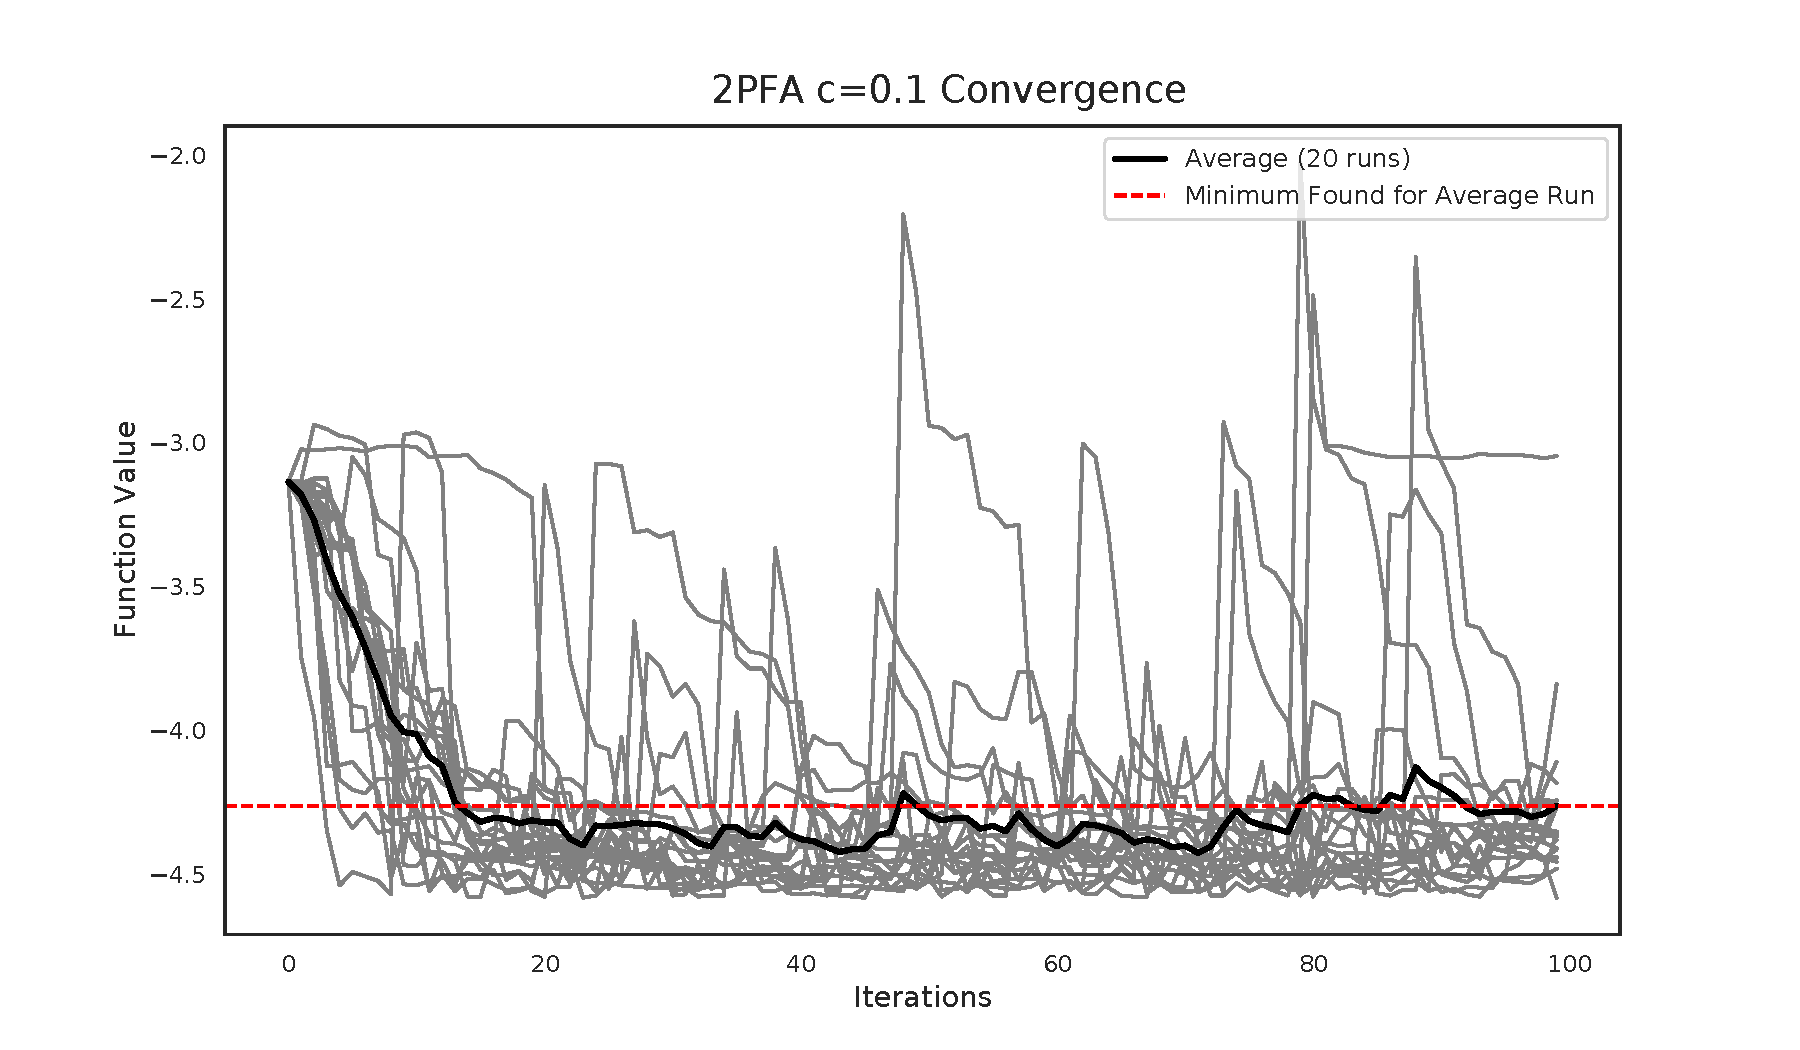
\includegraphics[width=0.32\linewidth]{figures/itercomp/cmp_2pfa_c01_a01.pdf}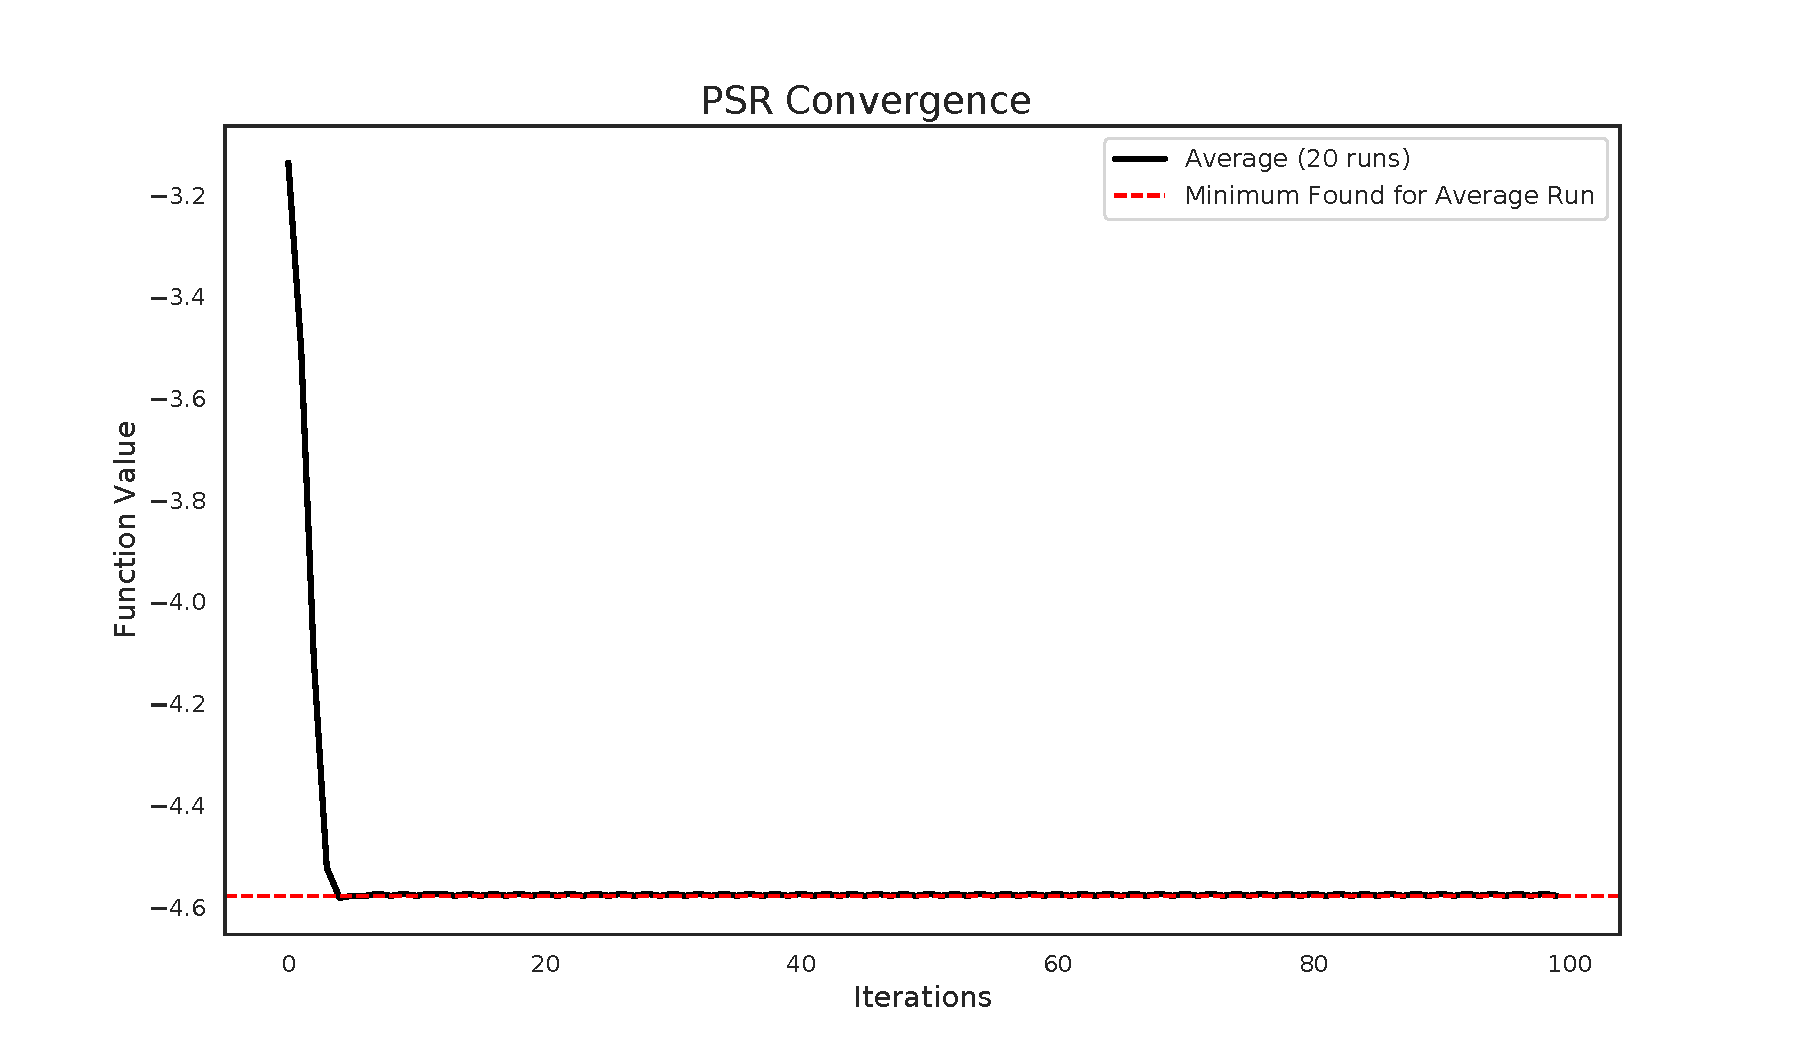
\includegraphics[width=0.32\linewidth]{figures/itercomp/cmp_psr_a01.pdf}\\
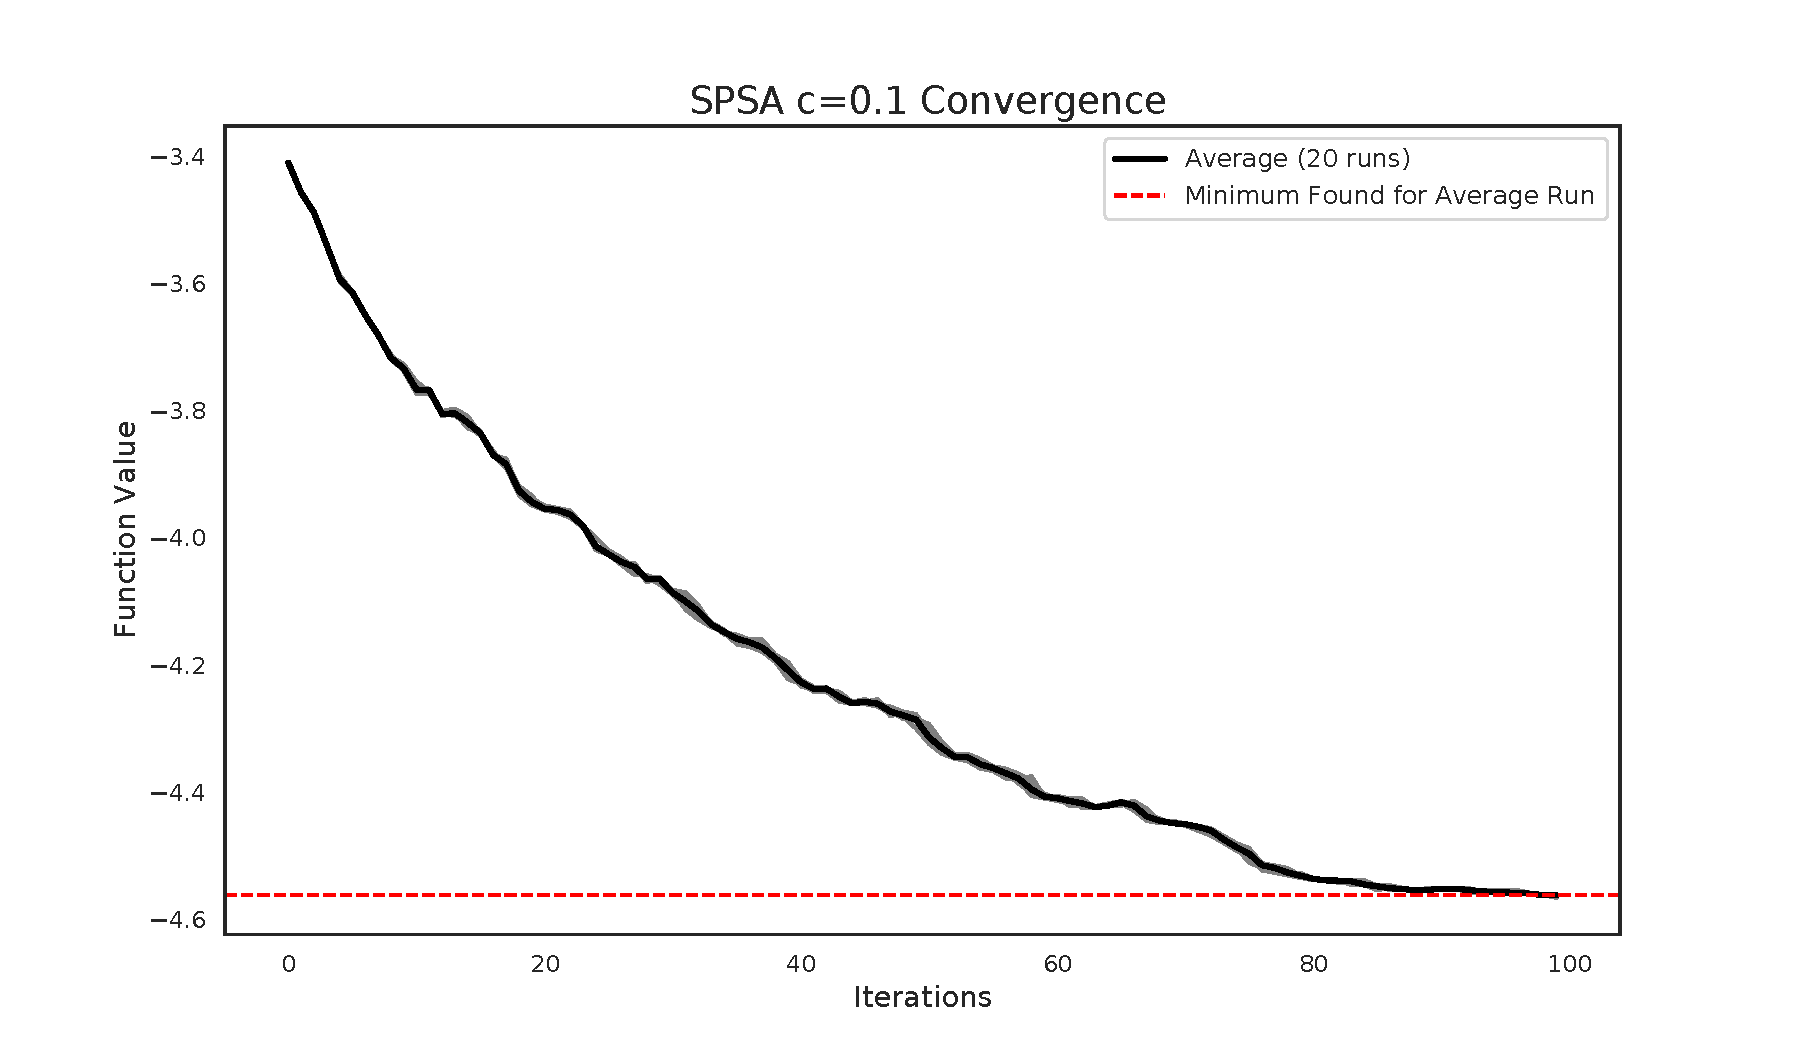
\includegraphics[width=0.32\linewidth]{figures/itercomp/cmp_spsa_c01_a0001.pdf}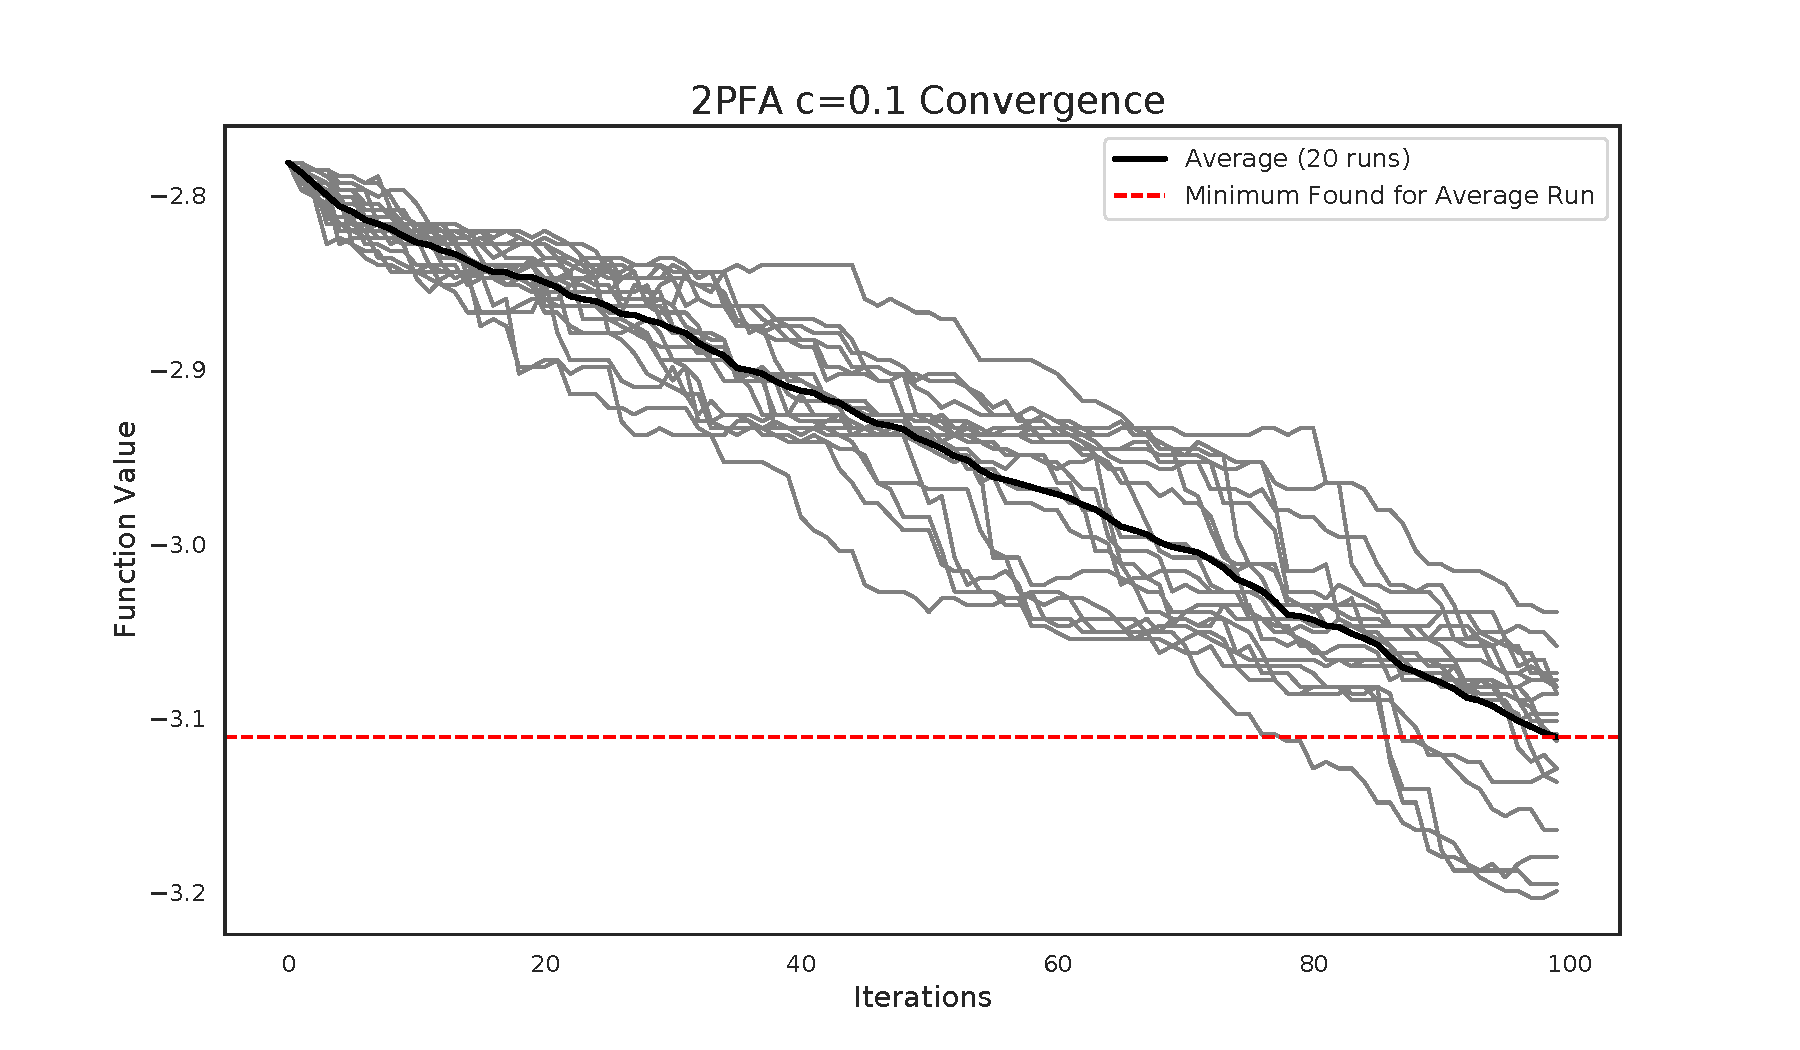
\includegraphics[width=0.32\linewidth]{figures/itercomp/cmp_2pfa_c01_a0001.pdf}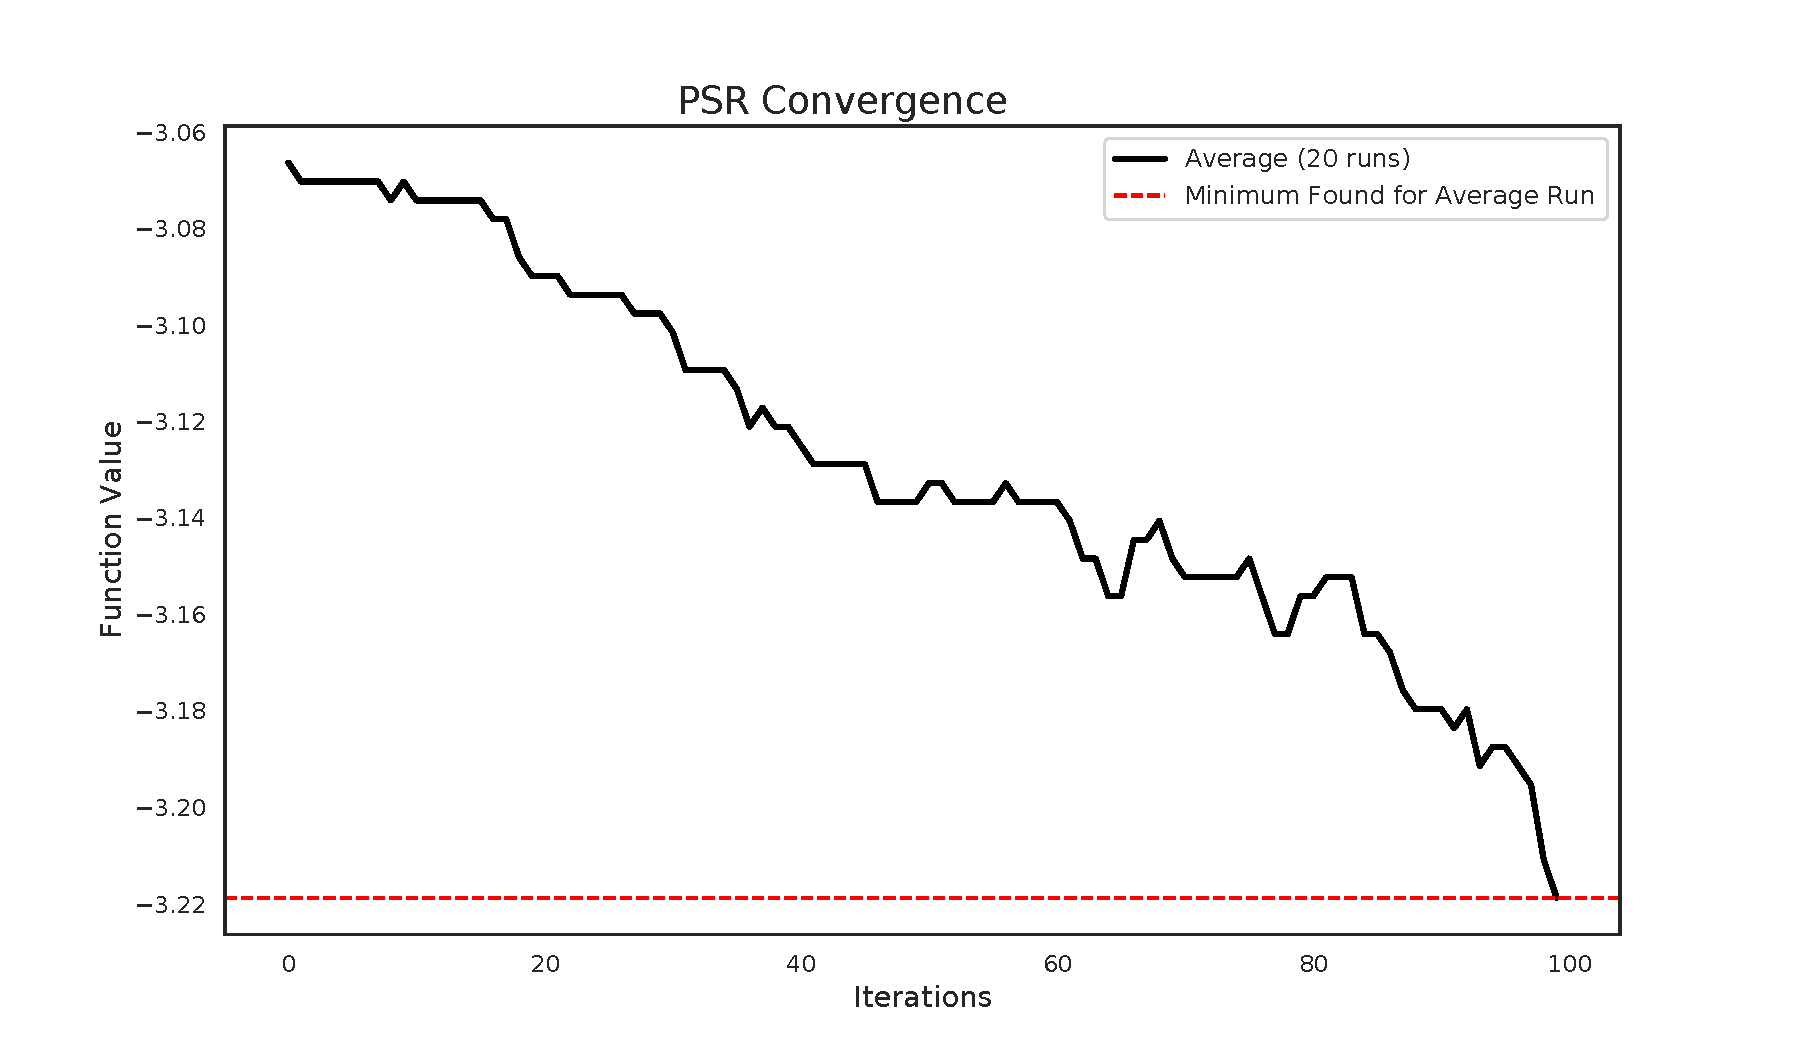
\includegraphics[width=0.32\linewidth]{figures/itercomp/cmp_psr_a0001.pdf}
\caption{Representative runs of SPSA (left), two-point approximation (centre) and parameter-shift rule (right) with perturbation $c = 0.1$; top row step size $\alpha = 0.1$, bottom row $\alpha = 0.001$ \cite{kungurtsev2022iteration}.}\label{fig:ch06:compare}\end{figure}}
\begin{itemize}\setlength\itemsep{0.1em}
    \item \emph{Large step, large perturbation:} SPSA converges as fast as the exact-gradient PSR, though to a noisier region with higher bias; 2PFA is slower and far less robust, with late iterates exceeding the starting value.
    \item \emph{Small step, large perturbation}, the safe regime: SPSA converges even faster than PSR; all three decrease steadily, 2PFA being the noisiest.
    \item \emph{Small perturbation} ($c \le 0.01$): SPSA becomes noisy with large steps; 2PFA becomes useless for $c = 0.001$, its variance swamping the steady decrease.
\end{itemize}
\end{frame}

\section{Discussion}

\begin{frame}\ft{Take-aways}
\begin{itemize}\setlength\itemsep{0.4em}
    \item \textbf{Bias does not change the rate} of convergence to stationarity; it enlarges the constants and imposes a floor: the more bias, the farther one is guaranteed, at best, to reach a stationary point.
    \item \textbf{Coarser gradient estimates stabilise against bias} but add their own approximation bias; there is an optimal perturbation $c^*(b, p)$.
    \item \textbf{Zero-order methods scale poorly with dimension} in the floor, as usual; SPSA is the most forgiving among them and is a reasonable default for VQAs, provided $c$ is not too small.
    \item \textbf{This is a small step} towards understanding variational methods beyond ``heuristics with no guarantees''; together with warm starts (\Chap~\chref{C.WSRounded}), which bound the objective at the limit point, one begins to characterise their performance.
    \item Open: relating the stationarity measure $\|\nabla f\|^2$ to the approximation ratio of the sampled solutions, which is what \Chap~\chref{C.PerIteration} measures empirically.
\end{itemize}
\end{frame}

\begin{frame}[allowframebreaks]\ft{References}
\biblio
\end{frame}

\end{document}
